% 文档类
\documentclass[13pt]{ctexart}
% 设置页面
\usepackage{geometry}
\usepackage{wrapfig}
% 插图片
\usepackage{graphicx}
% 设置标题 重命名为英文
\renewcommand{\figurename}{Figure}
\renewcommand{\tablename}{Table}
\renewcommand{\contentsname}{Contents}
% 设置摘要页缩减 
\usepackage{changepage}
% 便于修改字体
\usepackage{fontspec}
% 设置页眉页脚
\usepackage{fancyhdr}
% 清空页眉页脚
\pagestyle{fancy}
% 设置列表缩进
\usepackage[shortlabels]{enumitem}
% 设置修改默认的section标题大小
\usepackage{titlesec}
\titleformat*{\section}{\LARGE}
\titleformat*{\subsection}{\Large}
\titleformat*{\subsubsection}{\Large}
% 使用数学宏包
\usepackage{amsmath}
% 设置表格的列格式
\usepackage{array}
% 三线表宏包
\usepackage{booktabs}
% 设置产考文献不输出默认名
\usepackage{etoolbox}
\patchcmd{\thebibliography}{\section*{\refname}}{}{}{}
% 引入网站作为参考文献
\usepackage{url}
% 设置等宽的代码字体
\setmonofont{Courier New}
% 颜色
\usepackage{xcolor}
% 代码高亮方案宏包
\usepackage{listings}
\definecolor{CPPLight}  {HTML} {686868}
\definecolor{CPPSteel}  {HTML} {888888}
\definecolor{CPPDark}   {HTML} {262626}
\definecolor{CPPBlue}   {HTML} {4172A3}
\definecolor{CPPGreen}  {HTML} {487818}
\definecolor{CPPBrown}  {HTML} {A07040}
\definecolor{CPPRed}    {HTML} {AD4D3A}
\definecolor{CPPViolet} {HTML} {7040A0}
\definecolor{CPPGray}  {HTML} {B8B8B8}
\lstset{
	basicstyle=\ttfamily,
	breaklines=true,
	framextopmargin=50pt,
	frame=bottomline,
	columns=fixed,       
    %numbers=left,                                       % 在左侧显示行号
	frame=none,                                          % 不显示背景边框
	backgroundcolor=\color[RGB]{255,255,255},            % 设定背景颜色
	keywordstyle=\color[RGB]{40,40,255},                 % 设定关键字颜色
	numberstyle=\footnotesize\color{darkgray},           % 设定行号格式
	commentstyle=\itshape\color[RGB]{0,96,96},                % 设置代码注释的格式
	stringstyle=\slshape\color[RGB]{128,0,0},   % 设置字符串格式
	showstringspaces=false,                              % 不显示字符串中的空格
	language=python,                                     % 设置语言
	morekeywords={alignas,continute,friend,register,true,alignof,decltype,goto,
		reinterpret_cast,try,asm,defult,if,return,typedef,auto,delete,inline,short,
		typeid,bool,do,int,signed,typename,break,double,long,sizeof,union,case,
		dynamic_cast,mutable,static,unsigned,catch,else,namespace,static_assert,using,
		char,enum,new,static_cast,virtual,char16_t,char32_t,explict,noexcept,struct,
		void,export,nullptr,switch,volatile,class,extern,operator,template,wchar_t,
		const,false,private,this,while,constexpr,float,protected,thread_local,
		const_cast,for,public,throw,std},
	emph={map,set,multimap,multiset,unordered_map,unordered_set,numpy,graph,path,append,extend,
		unordered_multiset,unordered_multimap,vector,string,list,deque,
		array,stack,forwared_list,iostream,memory,shared_ptr,unique_ptr,
		random,bitset,ostream,istream,cout,cin,endl,move,default_random_engine,
		uniform_int_distribution,iterator,algorithm,functional,bing,numeric,},
	emphstyle=\color{CPPViolet}, 
}

\begin{document}
\newgeometry{top = 1cm, right = 2.54cm, left = 2.54cm, bottom = 2.54cm}
% 第一页的字体为times new roman
\setmainfont{Times New Roman}
\thispagestyle{empty}

\begin{table}[h]
    \quad { }  \begin{minipage}[t]{5.5cm}
        % arraystretch 是调节列高
        \begin{tabular}[t]{>{\centering\arraybackslash}b{10em}}
            \fontsize{12pt}{10pt}\selectfont \textbf{Problem Chosen}\\ [2pt]
            {\color{red} \fontsize{20pt}{10pt}\selectfont C}
        \end{tabular}
    \end{minipage}
    \begin{minipage}[t]{5.2cm}
        \begin{tabular}[t]{>{\centering\arraybackslash}p{10em}}
            \fontsize{12pt}{10pt}\selectfont \textbf{2024} \\ [-2pt]
            \fontsize{12pt}{10pt}\selectfont \textbf{MCM/ICM} \\ [-2pt]
            \fontsize{12pt}{10pt}\selectfont \textbf{Summary Sheet}
        \end{tabular}
    \end{minipage}
    \begin{minipage}[t]{3cm}
        \begin{tabular}[t]{>{\centering\arraybackslash}b{12em}}
            \fontsize{12pt}{10pt}\selectfont \textbf{Team Control Number} \\ [2pt]
            {\color{red} \fontsize{21pt}{10pt}\selectfont 2403370}
        \end{tabular}
    \end{minipage}
\end{table}
\vspace{-20pt}
\noindent{\rule{\textwidth}{0.5mm}}

% 标题
{\centering\fontsize{18}{16}\selectfont\textbf{{Momentum in Tennis Matches}}
% 摘要
\vspace{10pt} 

\fontsize{13}{10}\selectfont\textbf{{Summary}}\par}
\vspace{10pt}

% 正文字体 13 pt
\fontsize{13}{12.5}\selectfont

\begin{adjustwidth}{1cm}{1cm}
\indent { }{ }{ }{ }{ }{ }In the competitive realm of sports, understanding player momentum is key to deciphering match outcomes. Our research introduces the \textbf{Momentum-Swings Prediction Model}, a novel approach tailored for tennis, focusing on the intricate dance of mental and performance shifts. Aiming to offer a fresh lens through which to predict the unfolding narrative of tennis matches.

Prior to launching our models, we leverage the capabilities of \textbf{Backpropagation Neural Network} to conduct meticulous data preprocessing. Through the application of sophisticated visualization techniques, we guarantee that our nuanced analysis is not only \textbf{intuitive} but also eloquently \textbf{presented}.

For Model I: We first performed \textbf{data preprocessing} to remove anomalies or deviations from the data. Then, inspired by real sports experience, the \textbf{calculation method of momentum} was creatively proposed by combining psychological factors with strength factors. Finally, design a model that \textbf{reflects the player's performance} in the game through the momentum at each moment. Additionally, we conducted preliminary testing of the model using the 2023 men's Wimbledon round of 16 match (ID1301) between Alcaraz and Jarry.

For Model II: We have added a score gap line to the existing Model I and conducted \textbf{Pearson correlation test}. We validated the strong correlation between momentum and difference by calculating the \textbf{P-value} of the correlation and setting a threshold for significance level. This further highlights the important role of momentum in driving player success, and strongly \textbf{refutes some coaches' claim} that the relationship between momentum and success is random.

For Model III, we redefined swings as the \textbf{change in momentum}. Using \textbf{correlation coefficient matrices}, we analyzed momentum's correlation with various factors. This aids in identifying factors closely linked to momentum and extending the model to other competitions. After establishing the \textbf{Momentum-Swings Prediction Model}, we tested it on data not fully analyzed by Model II. Meeting expectations, we focused on Djokovic's 2023 Wimbledon final defeat. Finally, our team's local table tennis match data verified the model's \textbf{generalizability} with satisfactory results.

After testing, we considered the advantages and disadvantages of three models, and conducted stability testing using \textbf{LSTM testing}. Finally, a conclusion was provided, and suggestions were made to tennis coaches and athletes.

\vspace{15pt}
\textbf{key words} : momentum, swing, linear, correlation matrices, LSTM
\end{adjustwidth} 

% 开始写 memo 信
% 更换字体为 palatino 也可以不换
\setmainfont{TeX Gyre Pagella}
\newpage
\newgeometry{left = 3.5cm, right = 3.5cm}
\thispagestyle{empty}

{\centering \fontsize{18pt}{14pt}\selectfont \textbf{MEMO}\par}

\noindent FROM: Team {} 2403370 , MCM/ICM C

\noindent To: The group of coaches

\noindent Date: February 5, 2024

\vspace{10pt}

Dear Coaches:
It is our honor to help you with analyzing the role of momentum in competition. We are writing this letter to report our findings.

We analyzed the match process during scoring, and found that the probability of the server winning points/games is much higher. We also establish an analytical model to analyze the data of the entire match and determine the skill levels of the players on both sides. We found that despite Djokovic's high skill level, he still suffered defeat. This underscores the significance of momentum in tennis matches. Consequently, we introduced the concept of "momentum," which is quantified based on individual capabilities, psychological aspects, and real-time match situations. This approach allows us to weigh these factors and determine which player performs better at specific points in the game and to what extent.

We found a correlation between swings during the game and a player's success. Through graphical representations, it is visually evident that significant disparities in momentum lines between the two players correspond to substantial swings in the score difference lines, indicating their correlation. In terms of rigorous mathematical analysis, we utilized the Pearson correlation test. The calculated p-values and r-values demonstrate a close correlation between swings and a player's ability to succeed.

We have discovered indicators that can assist in determining when the dynamics of a game will shift from favoring one player to another. We established a mathematical model, synthesized data from several matches, analyzed, and identified the top five factors related to swings during the game. Furthermore, we found that the proportion of each factor influencing game swings may experience slight variations in each match. We have also established a model to predict the turning points of the game by forecasting momentum. According to this swing model, we recommend that athletes, prior to the competition, should, based on individual differences and trends in momentum swings, comprehensively consider psychological factors. Additionally, they should make real-time tactical adjustments to bring out their best performance during the game.

Based on our analysis, we provide some suggestions to effectively prepare players to respond to events that influence the rhythm of a tennis match:

1. Players and coaching teams should closely observe the opponent's performance, including their techniques, physical condition, and tactical choices. Reacting promptly to potential changes in the opponent's strategy is key to maintaining momentum in the match.

2. It is recommended that players maintain open and timely communication with their coaching team. Discussing observations and the opponent's performance during the match allows for the formulation of adaptive and effective tactical strategies.

3. As the game progresses, changes in the score can significantly impact the dynamics for both players. It is advisable to adjust tactics based on score changes, possibly requiring a more offensive or defensive approach to ensure the most favorable match momentum.

4. When making real-time tactical adjustments, factors such as the condition of the court surface, wind direction, and other weather elements should be taken into account. These factors can influence the trajectory and bounce of the ball, necessitating a comprehensive consideration during tactical adjustments.

5. Prior to the match, developing alternative tactical plans is essential. This enables players to quickly choose and execute alternative strategies when adjustments are needed during the game, facilitating better adaptation to the evolving situation.

We believe that our model is useful for preparing players to respond to events that influence the rhythm of a tennis match. You are welcome to contact us at any time for further cooperation.

% 信多出一页,清理页眉页脚
\thispagestyle{empty}
% 信的结尾
{\raggedleft
Sincerely yours

MCM/ICM C Team 2403370\par
}

% 目录页
\newpage
\thispagestyle{empty}
\small
\tableofcontents
\normalsize
\newpage
% 目录页后面是第一页
\setcounter{page}{1}

% 开始写正文
% 设置正文的页边距
\newgeometry{top=3cm, left=3.5cm, right=3.5cm}
% 设置正文的页眉页脚
\fancyhf{}
\fancyhead[C]{ }
% 此处修改右上角页码
\fancyhead[R]{Page \thepage\ of 20}
\fancyhead[L]{Team \# 2403370}
\fancyfoot[C]{\bfseries\thepage}
\textbf{\section{Introduction}}
\textbf{\subsection{Restatement of the Problem}}
The 2023 Wimbledon men's final was a spectacle, with the unexpected close score between the two players adding to its intensity. Even the dominant Djokovic experienced an unusual swing, ultimately resulting in his defeat and bringing an end to his legendary performance. In light of this unprecedented situation, there are several issues that need addressing:
\begin{itemize}
	\item Describing the progression of the game and assessing individual player performances at specific moments.
	\item Refuting the notion that "momentum" does not influence a player's success and establishing its relationship as non-random.
	\item Predict swings in the game, study when the game will begin to lean towards a specific player, and provide suggestions for players to play.
	\item Testing prediction stability and generalizability while composing a letter to the coach regarding preparation for complex events.
\end{itemize}
\textbf{\subsection{Our Works}}

\begin{itemize}
    \item Establish an analysis model to analyze the data of the entire game and determine the level of both players.
    \item Quantify the concept of "momentum" to measure the possible swings that may occur during the competition, and comprehensively analyze its relationship with player performance.
    \item Predict the time when the game begins to tilt based on the data, and test the stability of the model with more games.
    \item Extend the model to more games (such as women's games) and even other competitions (such as table tennis, chess, etc.).
\end{itemize}

\textbf{\section{Assumptions and Notations}}
\vspace*{-10pt}
\textbf{\subsection{Assumptions}}
\begin{itemize}
    \item The audience does not affect the performance of the players.
    \item The natural environment inside the stadium does not affect the performance of the players.
    \item The physical condition of the players is good.
    \item There are no unexpected events during the game.
\end{itemize}

\textbf{\subsection{Notations}}
Here are all the notations and their meanings in this paper.
\begin{table}[h]
	\centering
	\vspace{3pt}
	\begin{tabular}{>{\centering\arraybackslash}p{5em}>{\centering\arraybackslash}p{30em}}
	\toprule % 绘制第一条线
	Symbol & Meaning \\ \midrule
    $M_s$ & Total momentum\\
    $M_b$ & Basic momentum\\
    $M_c$ & Change momentum\\
    $S_n$ & Game ratio\\
    $W_n$ & Winning games\\ 
    $S_e$ & Serving first\\
    $S_g$ & Score gap\\ 
    $v$ & Ball speed\\
    $S_p$ & Score per game\\
    $W_b$ & Winning shots\\
    $A_c$ & Winning serves\\
    $D_f$ & Double faults\\ 
    $U_e$ & Unforced errors\\ 
    $S$ & Swings\\ 
    $T$ & Swings threshold\\ 
    $\alpha, \beta$ & Constants\\ 
	\bottomrule
	\end{tabular}
\end{table}

\textbf{\section{Model Construction and Analysis}}
Before starting the model construction, we first preprocessed the data. Among this, the handling of outliers is particularly crucial.

We selected all fields of numerical types and calculated the mean and standard deviation for each field. Then we used three times the standard deviation from the mean as the threshold to define outliers. Once outliers were identified, we replaced them with NaN to avoid data loss. Although this created new missing values, we addressed this issue through forward and backward filling strategies. This strategy is commonly used in time series data and can maintain the overall trend of the data. After this treatment, we successfully corrected the outliers in the data, which helps to improve the accuracy of the model.
\textbf{\subsection{Momentum Model for Local Performance Analysis}}
To better analyze the "momentum" of a player at a certain moment, we introduced a term "momentum", which is defined in the dictionary as "strength or force gained by motion or by a series of events"[1]. In sports, momentum often manifests as athletes being full of confidence and strength during a match. It is obvious that momentum is closely related to the performance of the player, and is usually positively correlated. We decided to use momentum to determine the performance of the player. However, this kind of momentum is actually difficult to measure because it is often instantaneous and psychological. Therefore, we proposed a simulation method.

\textbf{\subsubsection{How to Calculate Momentum?}}
As we all know, playing a match is not only a test of the player's strength, but also a huge test of the player's psychological quality.

Therefore, both the player's strength and psychology should be part of the momentum. Correspondingly, there are some changes in momentum, such as when a player hits a winning ball, or makes a big mistake, which not only affects the psychology, but also may affect the player's strength. Therefore, we classify this situation as changing momentum, and the original momentum is called basic momentum. The total momentum is the sum of these two.

\begin{equation}
    M_s=M_b+M_c
\end{equation}
\\
\textbf{Basic Momentum}
~~On the psychological level, first, when a player gets more points after fewer rounds, or gets fewer points after more rounds, his psychology will inevitably undergo a huge change. Therefore, we introduced the definition of the round-to-point ratio, which can to some extent show the relationship between points and rounds, and indirectly reflect part of the player's psychology. Secondly, aside from the score, the number of rounds a player wins will also affect his psychology, making him more eager to win, and the momentum changes accordingly. Furthermore, if the point difference between the two players is large, it will also create a sense of crisis for both players. Finally, if a player serves first, his confidence must be higher than the other player who serves later. These four factors each account for 25\%, together constituting the psychological part of the basic momentum, to which we assigned a weight of α=45\%.
On the strength level, first, the simplest way to judge strength is the player's score per round, the higher the score, the stronger the player must be. Secondly, if a player can hit more winning balls, it can also indicate his level of strength. Finally, a more subtle point is that if a player is stronger, he generally has a higher average ball speed than others, which indicates that he has a better mastery of tennis and the racket (Figure 1).

\begin{figure}
    \centering % Centered display
    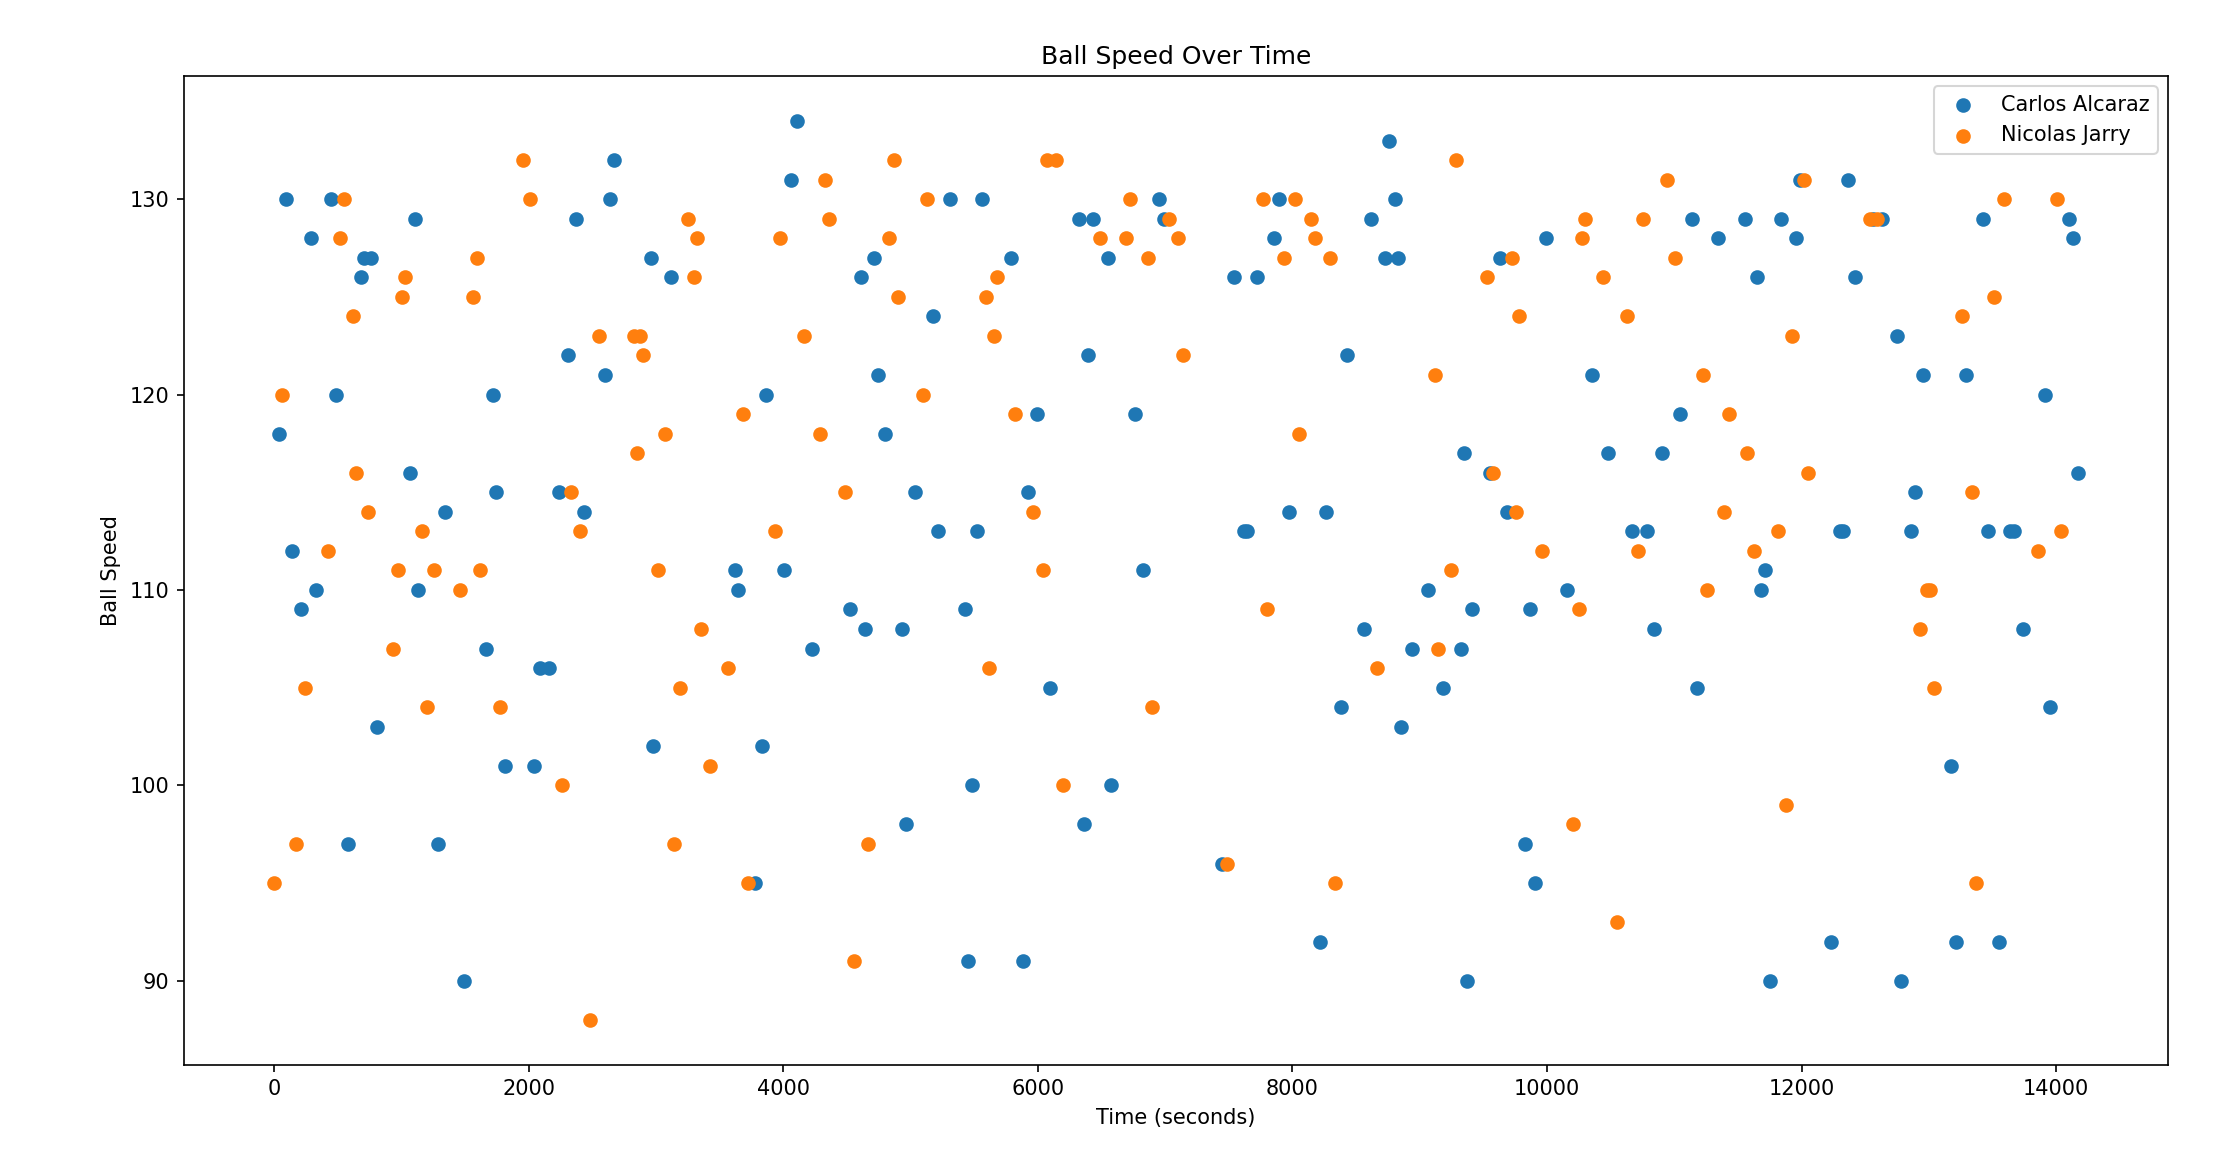
\includegraphics[width=13cm,height=7cm]{Ball speed.png}
    \caption{Ball speed of both players in match 1301} % Title
\end{figure}

These three aspects each account for 33.3\%, together constituting the strength part of the basic momentum, to which we assigned a weight of β=55\%.

\begin{equation}
	\begin{aligned}
		M_b=\alpha(S_n+W_n+S_e+S_p) \cdot 25\%+\beta(v+S_p+W_b) \cdot 33.3\% \\
		\alpha=45\% \quad \beta = 55\% \quad \quad  \quad \quad \quad \quad \quad \quad
	\end{aligned}
	\end{equation}
\\
\textbf{Change Momentum}
~~The situation on the field is not constant, sometimes the performance of the players will change under the dual effects of psychology and strength. We have selected a few representative aspects, such as winning serves, double faults, and unforced errors. These situations are difficult to explain with the player's psychology or strength, so they are considered as changing momentum. We assume that the initial values of the three are all 0, and if one occurs, add 2. The expression is:
\begin{equation}
    M_c=A_c-D_f-U_e
\end{equation}
\\
Through the above calculations, we can get the player's \textbf{total momentum}
\begin{equation}
    \begin{aligned}
    M_s=\alpha(S_n+W_n+S_e+S_p) \cdot 25\%+\beta(v+S_p+W_b) \cdot 33.3\%+A_c-D_f-U_e\\
    \alpha=45\% \quad \beta = 55\% \quad \quad \quad \quad \quad \quad \quad \quad \quad \quad \quad \quad
    \end{aligned}
\end{equation}
\\
The above multiple data participate in the calculation of momentum, which is enough to basically reflect the player's performance in the game.

\textbf{\subsubsection{Model Testing}}
We take the match with ID 1301 as an example of this model. The two players are Carlos Alcaraz and Nicolas Jarry. The momentum during the match is shown in Figure 2.

\begin{figure}[h]
    \centering % Centered display
    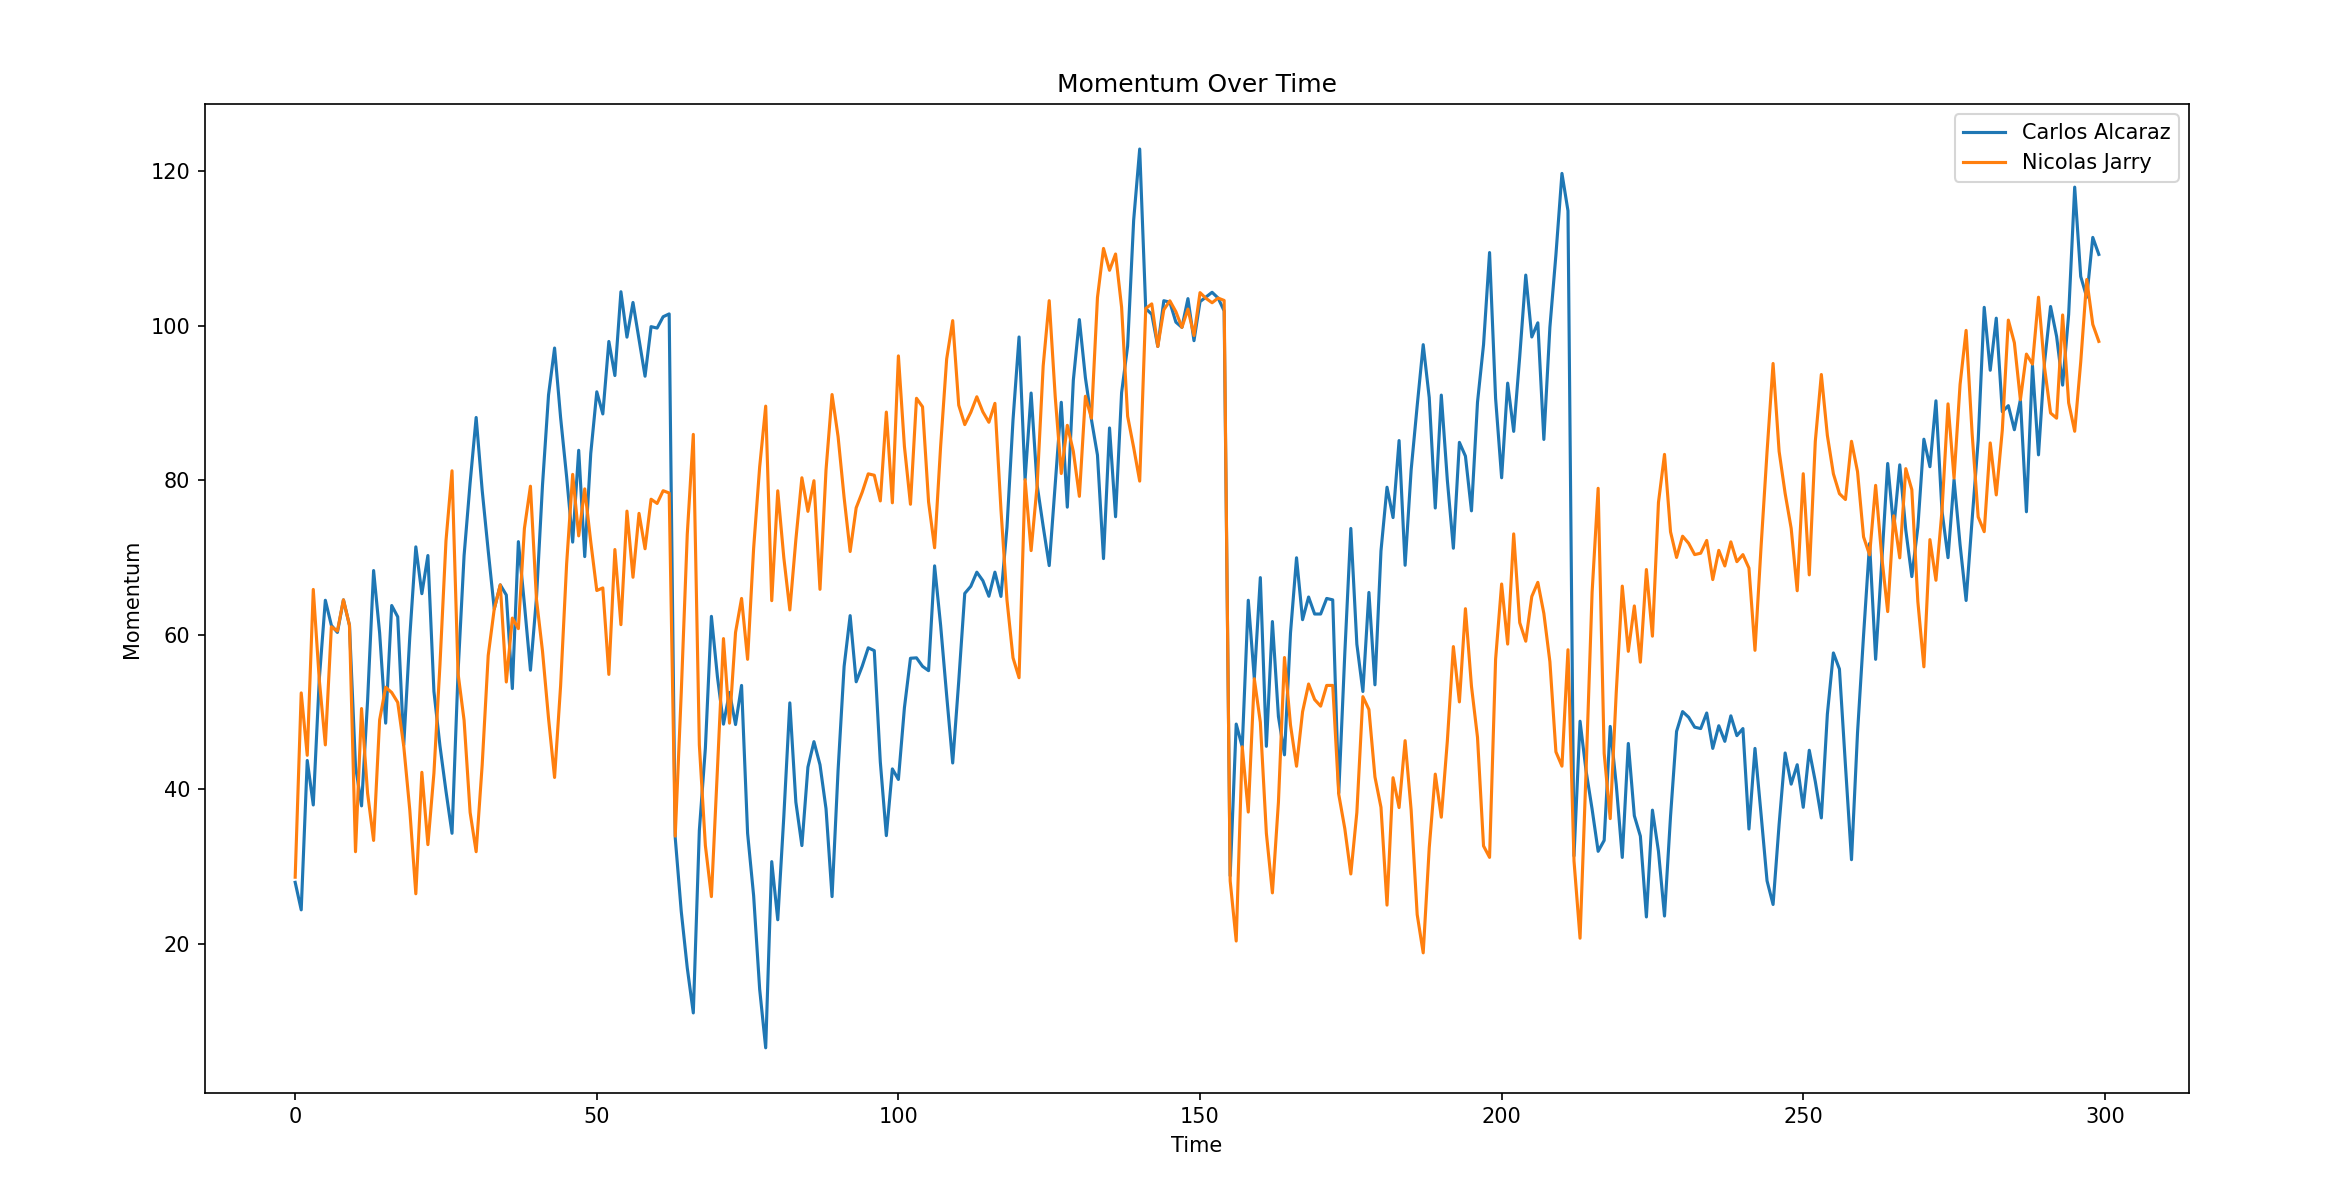
\includegraphics[width=13cm,height=7cm]{1301 momentum.png}
    \caption{Momentum of both players in match 1301} % Title
\end{figure}

The performance of the two at different stages of the match is clear at a glance. Among them, Alcaraz's performance fluctuates more, but the highest level is higher. The two compete for the upper hand repeatedly, and in the end, Alcaraz slightly wins and takes the victory of the match.
\textbf{\subsection{Momentum-Score Gap Correlation Test Model}}
A coach does not believe in the propelling effect of momentum on players. On the contrary, he believes that swings and whether a player can succeed are completely random. This is of course a completely wrong view, and we have given reasons to refute it.

For convenience, we still take the match 1301 as an example. Figure 3 adds a score gap line  to make it easier to analyze the situation.

\begin{figure}[h]
	\centering % 居中显示
	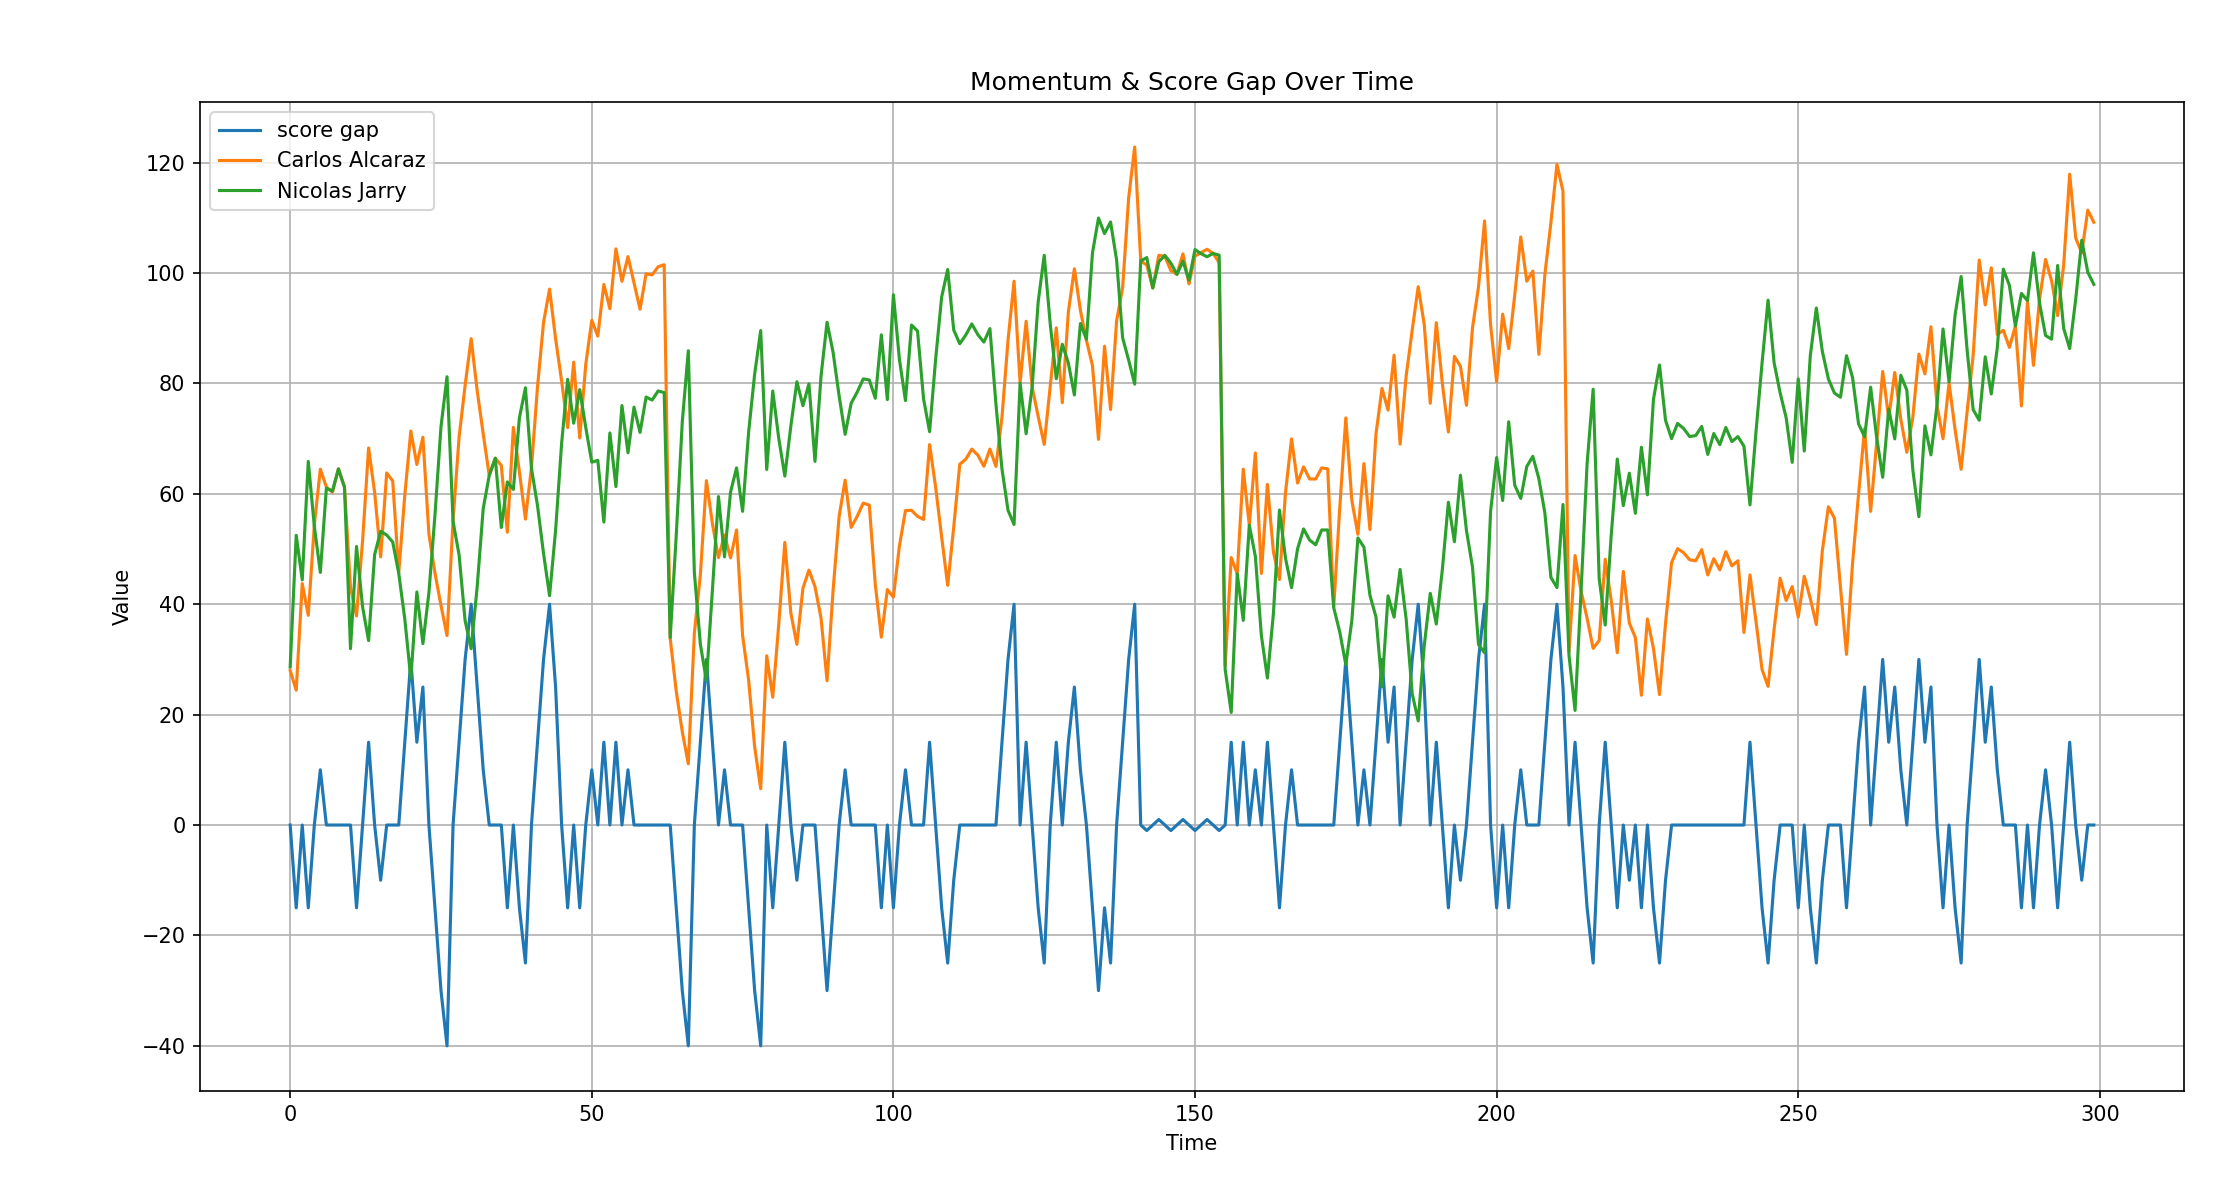
\includegraphics[width=15cm,height=6.5cm]{Refute the coach I.png}
	\caption{Momentum and score gap} % 标题
\end{figure}

\textbf{\subsubsection{Visual Observation}}
Looking at the places where the momentum lines of the two players differ greatly, obviously, the corresponding score difference line also has a lot of ups and downs, such as at time 50 and 200, the human eye and intuition can tell us that momentum and the situation of the match are strongly related. At the same time, the change in momentum is naturally one of the necessary conditions for swings to occur. Therefore, it can be said that swings and whether a player can succeed are closely related.

\textbf{\subsubsection{Pearson Correlation Test}}
We know that the simplest way to test whether two sets of data are related is the Pearson correlation test[2]. We use the P-values of the Permutation tests in it, that is, we judge the correlation of data through P-values. We set the threshold for the P-value at 0.001 to ensure the validity of the test. We used Python's mathematical analysis library to calculate the P-values and generated Figure 4, adding the relevant content of the Pearson correlation test based on Figure 3.
\begin{figure}[h]
\centering % 居中显示
	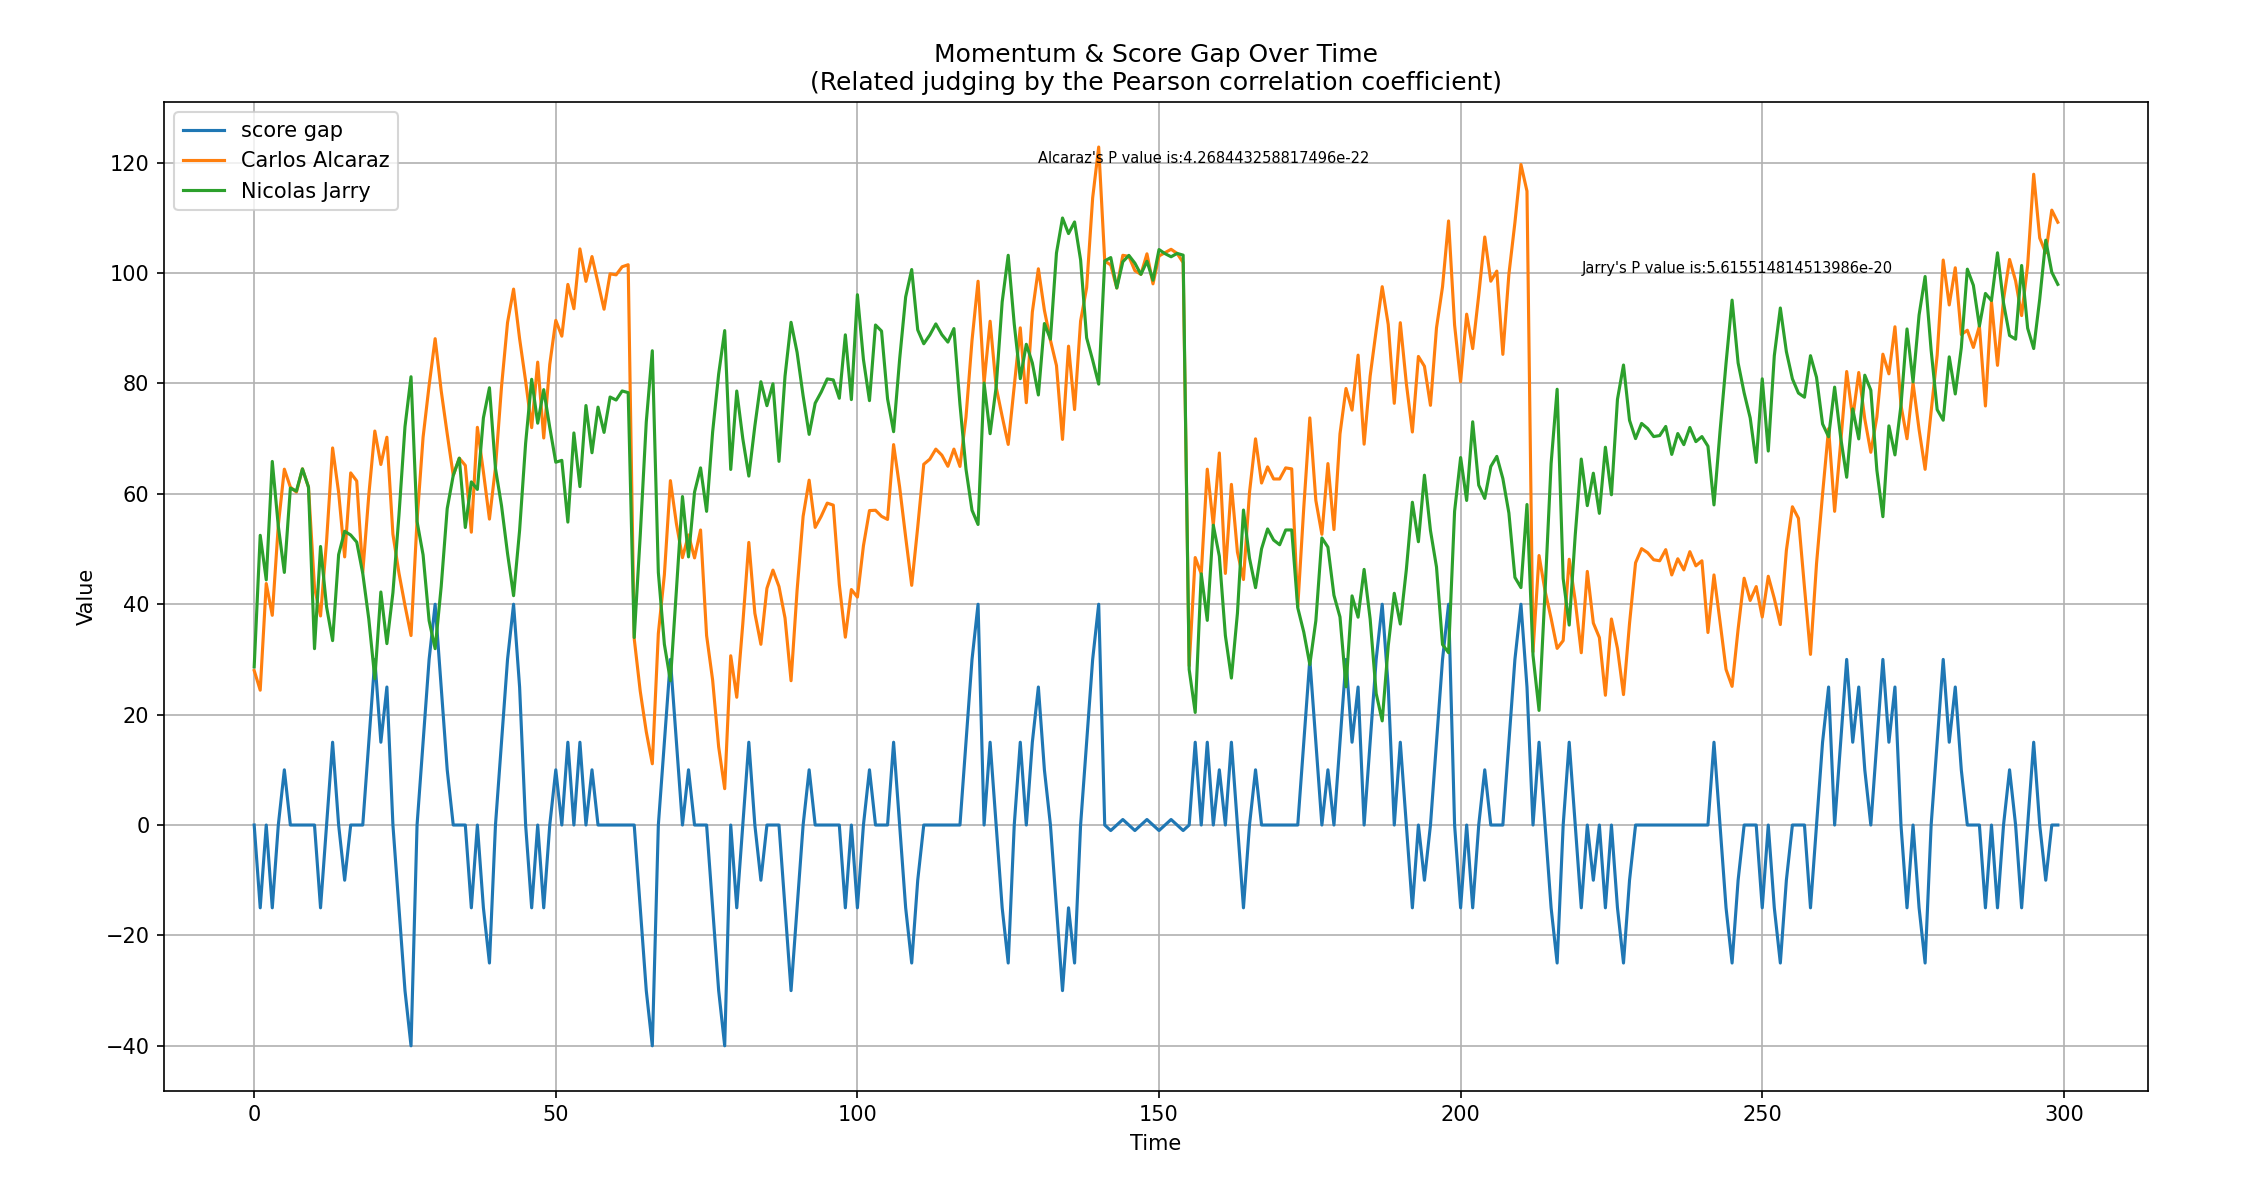
\includegraphics[width=15cm,height=7cm]{Refute the coach II.png}
	\caption{Correlation between momentum and score gap (P-value marked)} % 标题
\end{figure}

Clearly, the calculated P-value is far less than the threshold we set, indicating a very strong correlation between momentum and score gap. The Pearson correlation test refutes the coach's assertion more powerfully than the naked eye observation. From this, it can be understood that our model and inference are completely correct.

\textbf{\subsection{Momentum-Swings Prediction Model}}
Due to the instability of momentum, it is easily affected by various factors, and it has a crucial decisive role in the game. Coaches want to know when the game situation will fluctuate or even reverse.

\textbf{\subsubsection{How to Define Swings?}}
We analyzed the five most important factors affecting swings through match 1301, and then designed a momentum-swings prediction model to predict when players will swing in the match.

In order to quantify the concept of swings, we decided to regard it as a sudden change in momentum. In sections 3.1 and 3.2, we have verified that momentum is an indicator of a player's performance during a match. Therefore, the sudden change point of momentum is the sudden change point of a player's performance, which is also the generation point of swings. The turning point of a match exists among many swing points.

We give the formula:

\begin{equation}
	S=\frac{dM}{dt}
\end{equation}

\textbf{\subsubsection{What Factors Influence Swings Most?}}
As can be seen from the formula, swings are related to momentum, and swings are a reflection of changes in momentum. Therefore, we need to find the answer in the definition of momentum. However, momentum is determined by ten factors: the ratio of games, winning games, serving first, score difference, ball speed, scoring per game, winning balls, winning serves, double faults, and unforced errors. We cannot simply attribute these ten factors as the main reasons for causing swings. Therefore, we decided to select the four most important ones and continue to screen.

Put the ten factors into a table, calculate the correlation coefficient r between each pair, and regard it as a matrix, extract the relationship between the momentum of the two players and other factors, select the four factors with the largest correlation coefficient r, and draw them into a bar chart, as shown in Figure 5.

\begin{figure}[h]
	\centering % 居中显示
	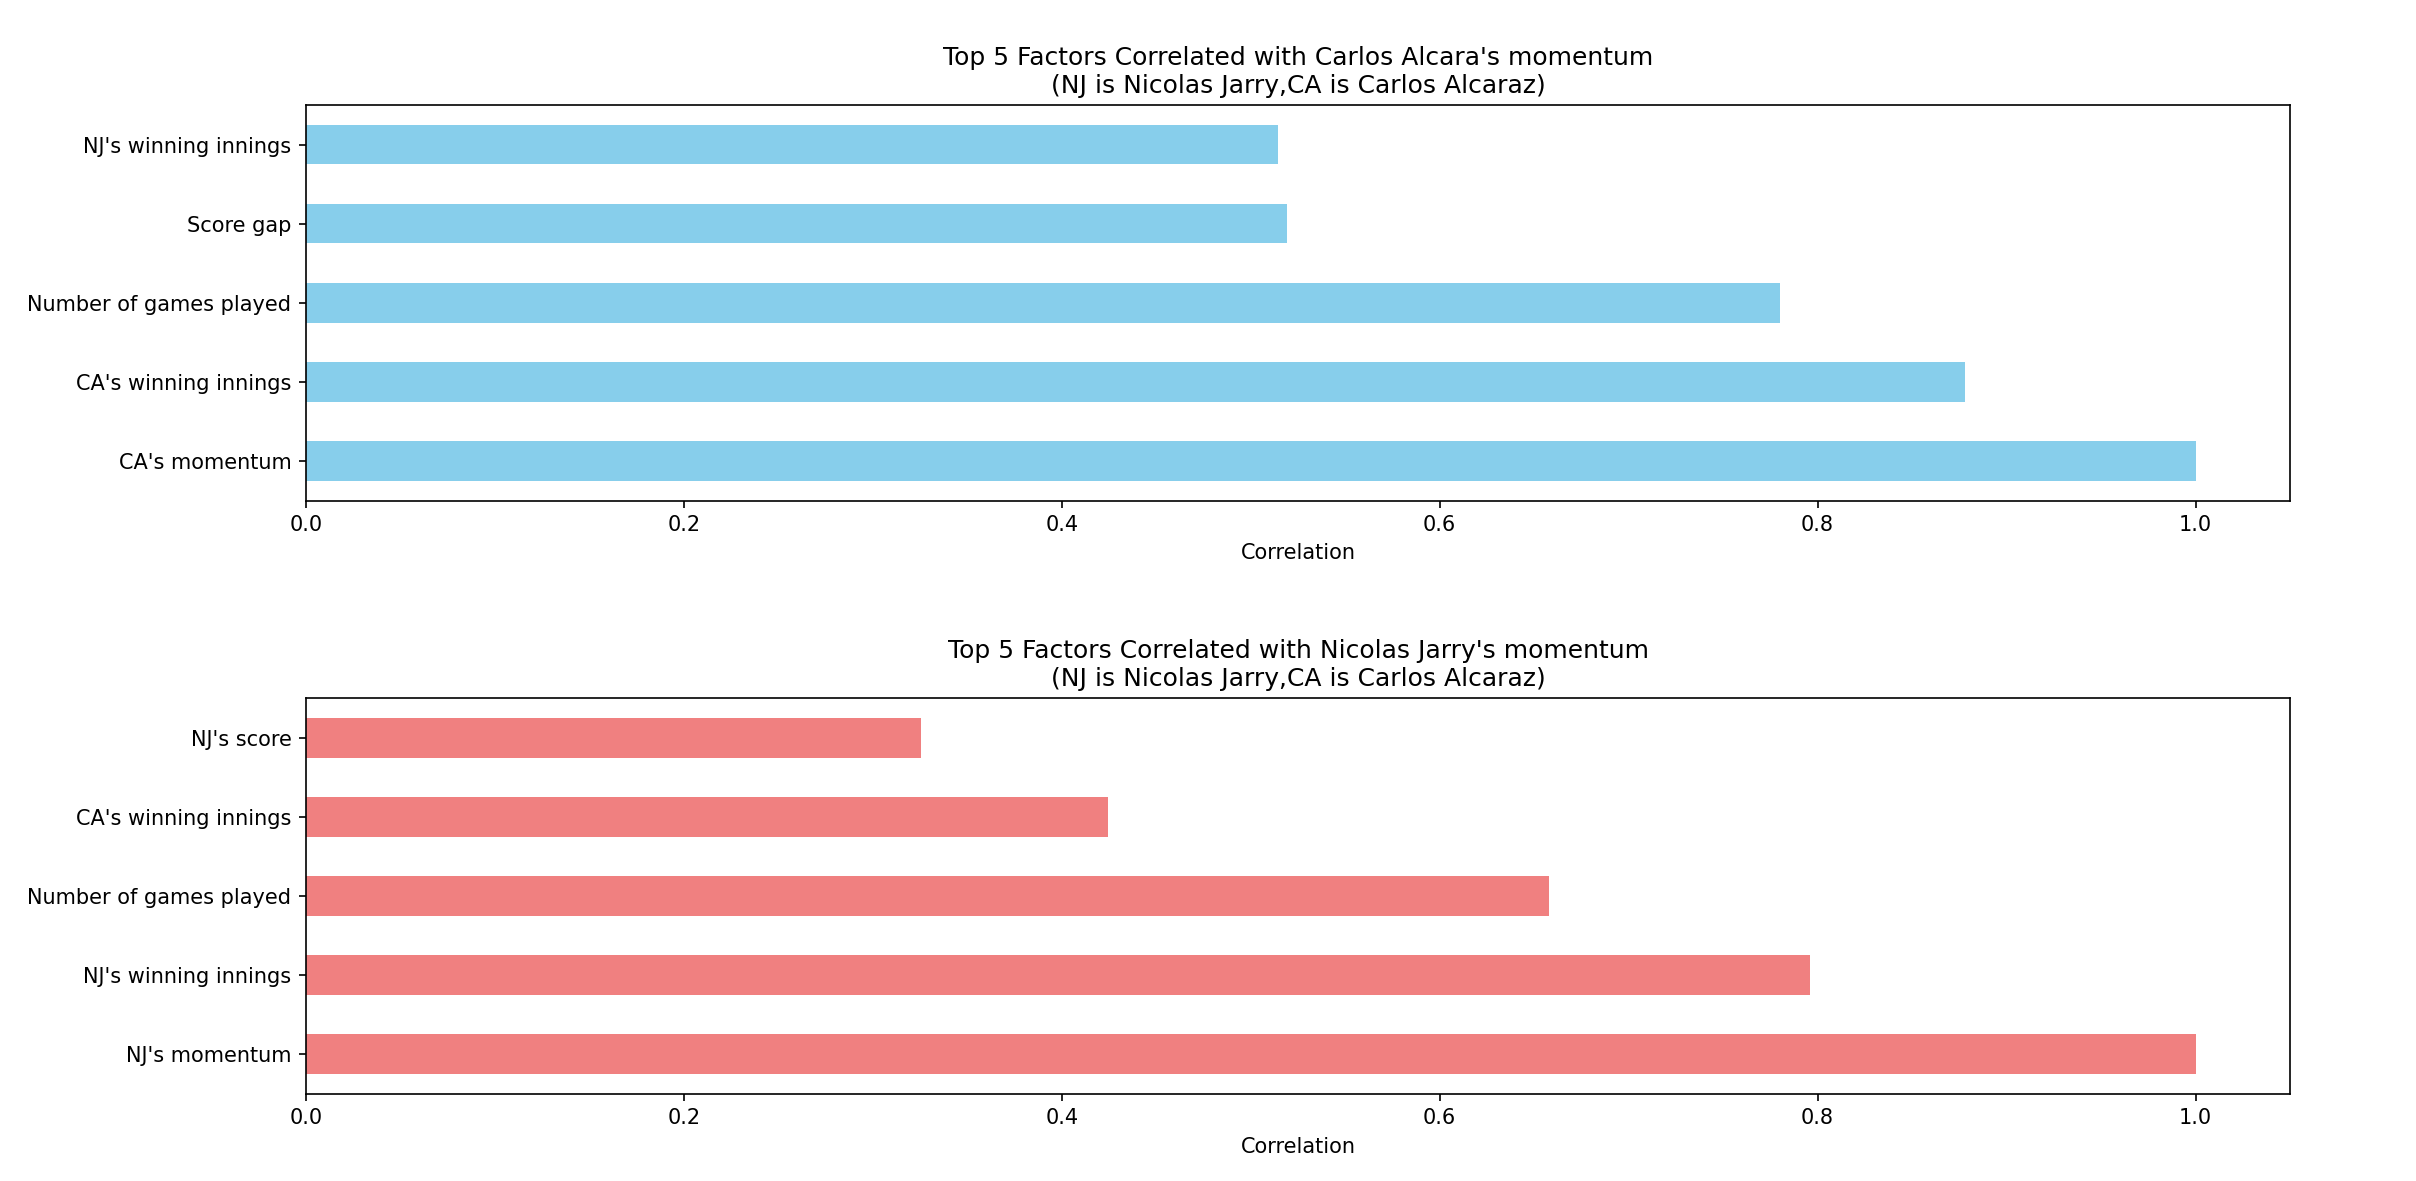
\includegraphics[width=15cm,height=8cm]{5 factors.png}
	\caption{Top 5 factors correlated with CA's momentum} % 标题
\end{figure}

The figure shows five factors. In fact, the factor with a correlation coefficient of 1 is momentum itself (it must be completely related to itself), so there are four most relevant factors. In addition, the factors of the two players are not exactly the same, which is caused by individual differences, model errors, etc. We can see from it that the correlation of the opponent's winning games and the total number of games played is greater than 0.6, so it can be judged that these two factors are most closely related to swings. (In other words, when one player thinks of the other's winning games and total games, it will inevitably have a greater impact on their psychology)

\textbf{\subsubsection{Model Construction}}
Due to the different strengths and psychological factors of the players, there will also be random and unpredictable situations in each match, so the change in momentum is normal to a certain extent. Therefore, we define a swing threshold $T=20$. When the change in momentum is greater than the swing threshold, record this moment as a swing point. And compile the momentum changes of a complete game into a chart, marking the swing points, among which the largest swing is the turning point.

Figure 6 is still an example of match 1301, and we chose Carlos Alcaraz as the analysis object.

\begin{figure}[h]
	\centering % 居中显示
	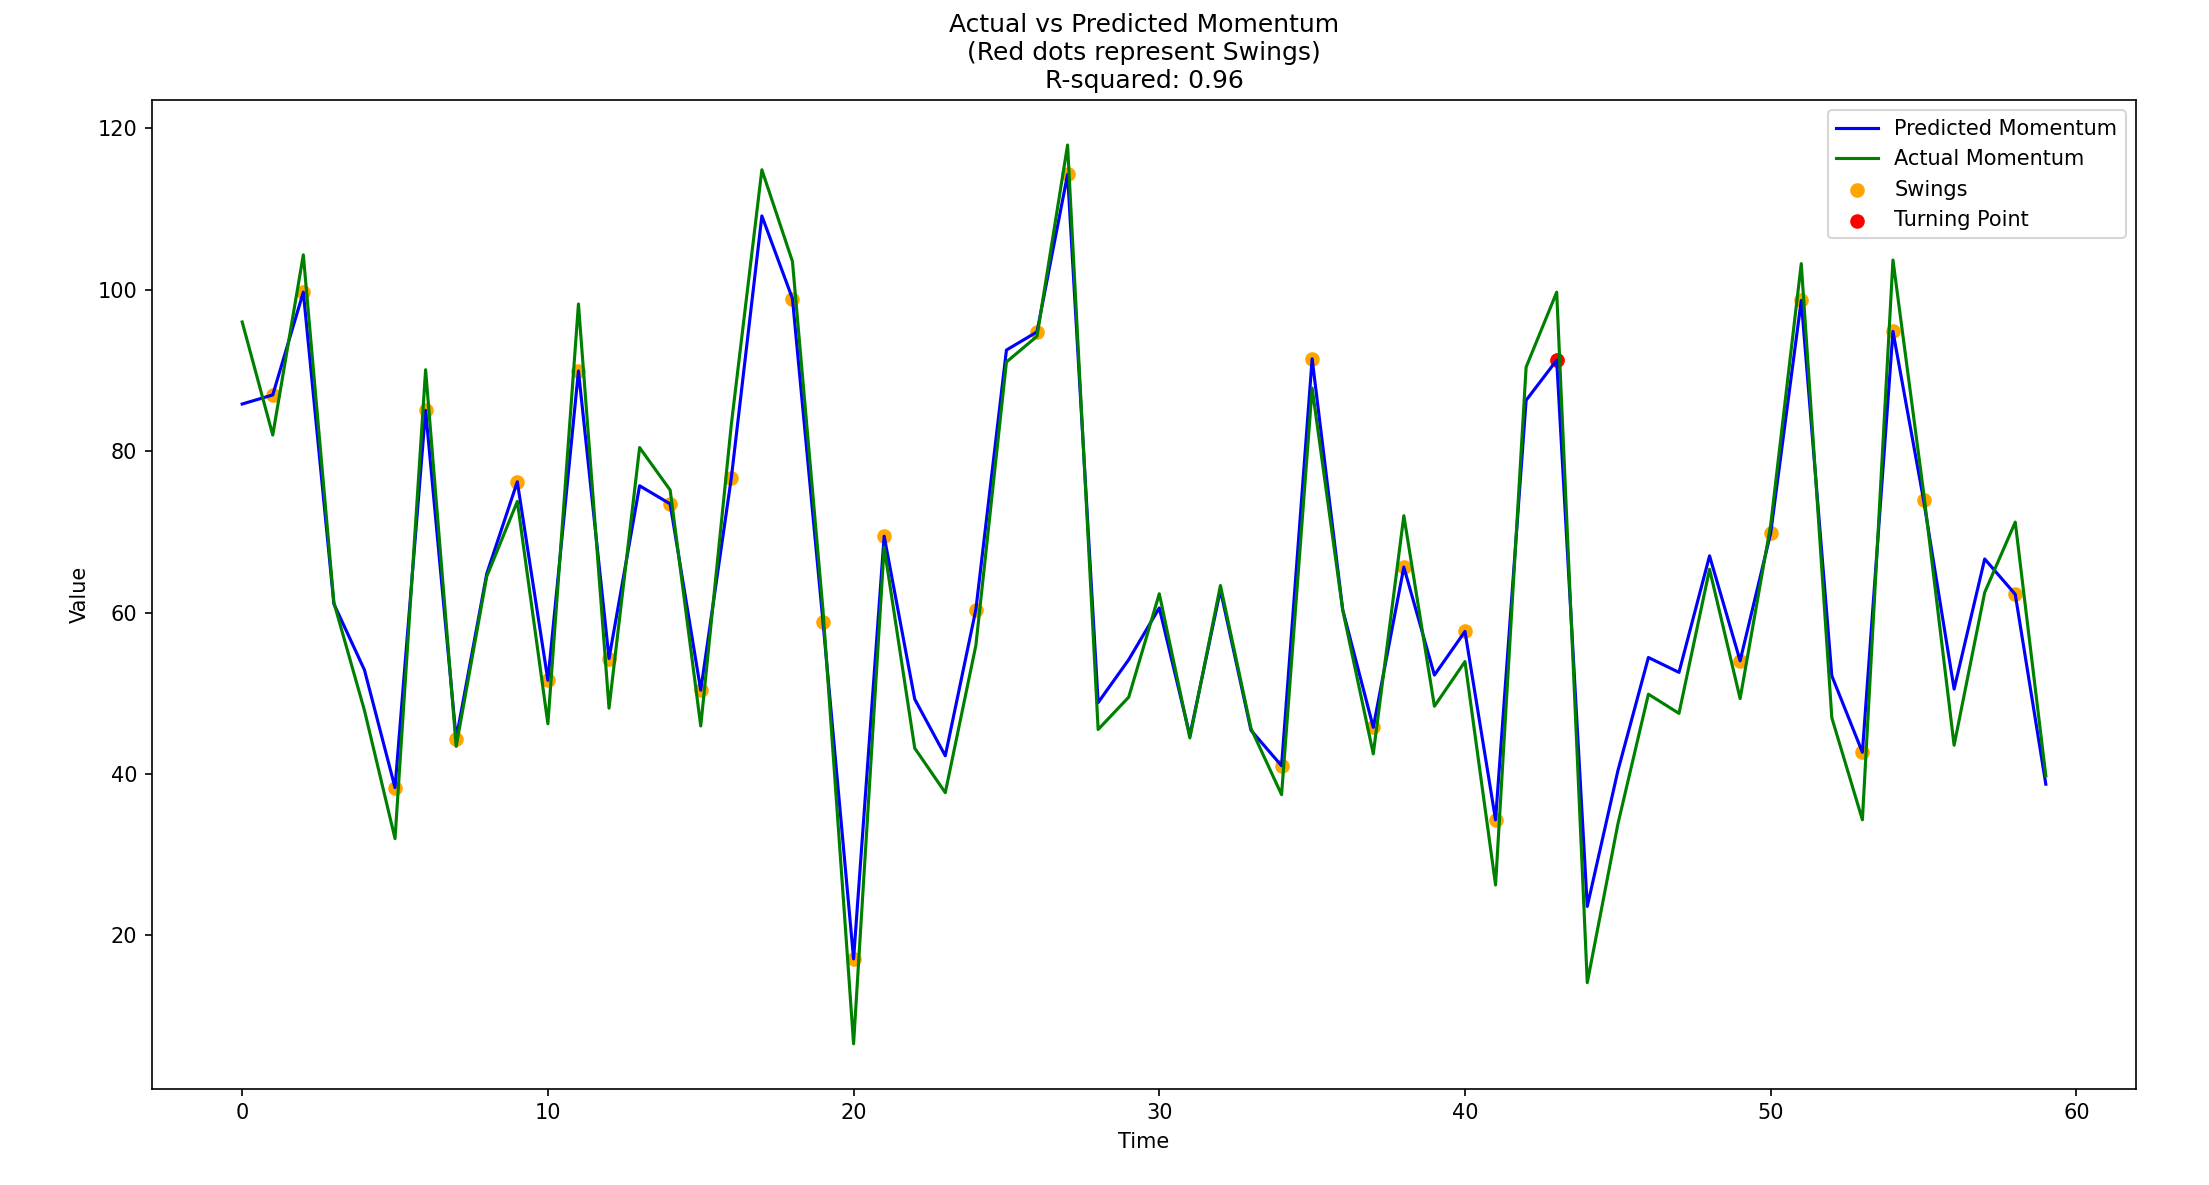
\includegraphics[width=15cm,height=8cm]{Swings Prediction.png}
	\caption{Predicting momentum changes and actual momentum changes, swings and turning points} % 标题
\end{figure}

We not only simulated the changes in momentum, predicted the swings, but also predicted the turning points of the match, and calculated the determination coefficient $R^2$ through the Pearson correlation test. The closer $R^2$ is to 1, the better the fit. 0.98 proves that after a large amount of data training, our model prediction results are very close to the actual situation.

The global changes in momentum (Alcaraz's performance) are clearly visible, where the orange part is the time point when he swings, and the red part is the turning point of this match. Fortunately, Alcaraz did not fall into despair after the turning point, but tried to maintain his state, and finally won after several large swings.

\textbf{\subsection{Suggestions}}
Considering the important role of momentum in the game and the huge impact of swings, we have given the following five suggestions to players and coaches.
\begin{itemize}
    \item Comprehensive analysis of individual differences: Before formulating game strategies, it is necessary to conduct an in-depth analysis of each athlete's individual characteristics and past game performance. In addition to identifying the factors that have the greatest impact on the opponent's "momentum" in the game, it is also necessary to consider factors such as the athlete's physical fitness, skills, and psychological state, to simulate potential factors that may have a positive impact on their "momentum".
    \item Detailed analysis of momentum swings trends: Use the momentum swings data in historical games to conduct a detailed trend analysis. This may involve quantitative and statistical analysis of the specific performance of "momentum" in each game, to reveal the patterns of "momentum" swings of different players in various scenarios.
    \item Individualized tactical suggestions: Based on individual differences and momentum swing trends, provide personalized tactical suggestions for each athlete. For players who focus on competitiveness, it is recommended to focus on maintaining a leading position in the game to fully utilize their positive attitude towards competition. For players who pay attention to the impact of opponents, it is recommended to pay attention to the performance of opponents and formulate corresponding countermeasures to maximize the weakening of the opponent's "momentum".
    \item Comprehensive consideration of psychological factors: Considering individual differences, especially the impact of psychological quality on the game's "momentum", it is recommended to conduct psychological training before the game. This may include training in emotion management, concentration, maintaining a good psychological state, etc., to improve the athlete's ability to cope with momentum swings in the game.
    \item Real-time tactical adjustments: Emphasize real-time observation and tactical adjustments during the game. Since the situation in the game may change at any time, it is recommended that athletes and coaching teams work closely together, flexibly adjust tactics according to the actual situation, to make the most of or counterbalance the swings of "momentum".
\end{itemize}

\textbf{\section{Further Testing}}
So far, our model has only used data from match 1301. One match cannot explain everything, we need to test more match data to verify the accuracy of the model, if the simulation effect is not good, we need to determine the cause of the problem and the solution. Additionally, we need to test the model's generalizability as much as possible, such as the performance of the model in various events such as women's tennis matches, table tennis, badminton, etc.

\textbf{\subsection{Why Djokovic lose?}}
Returning to the beginning of the article, why would Djokovic, a veteran who has been in the limelight, lose to a young man who is not well-known? Our model can well explain why Djokovic lost the match. Figure 7 is the momentum chart of his final with Alcaraz.

\begin{figure}[h]
    \centering % Centered display
    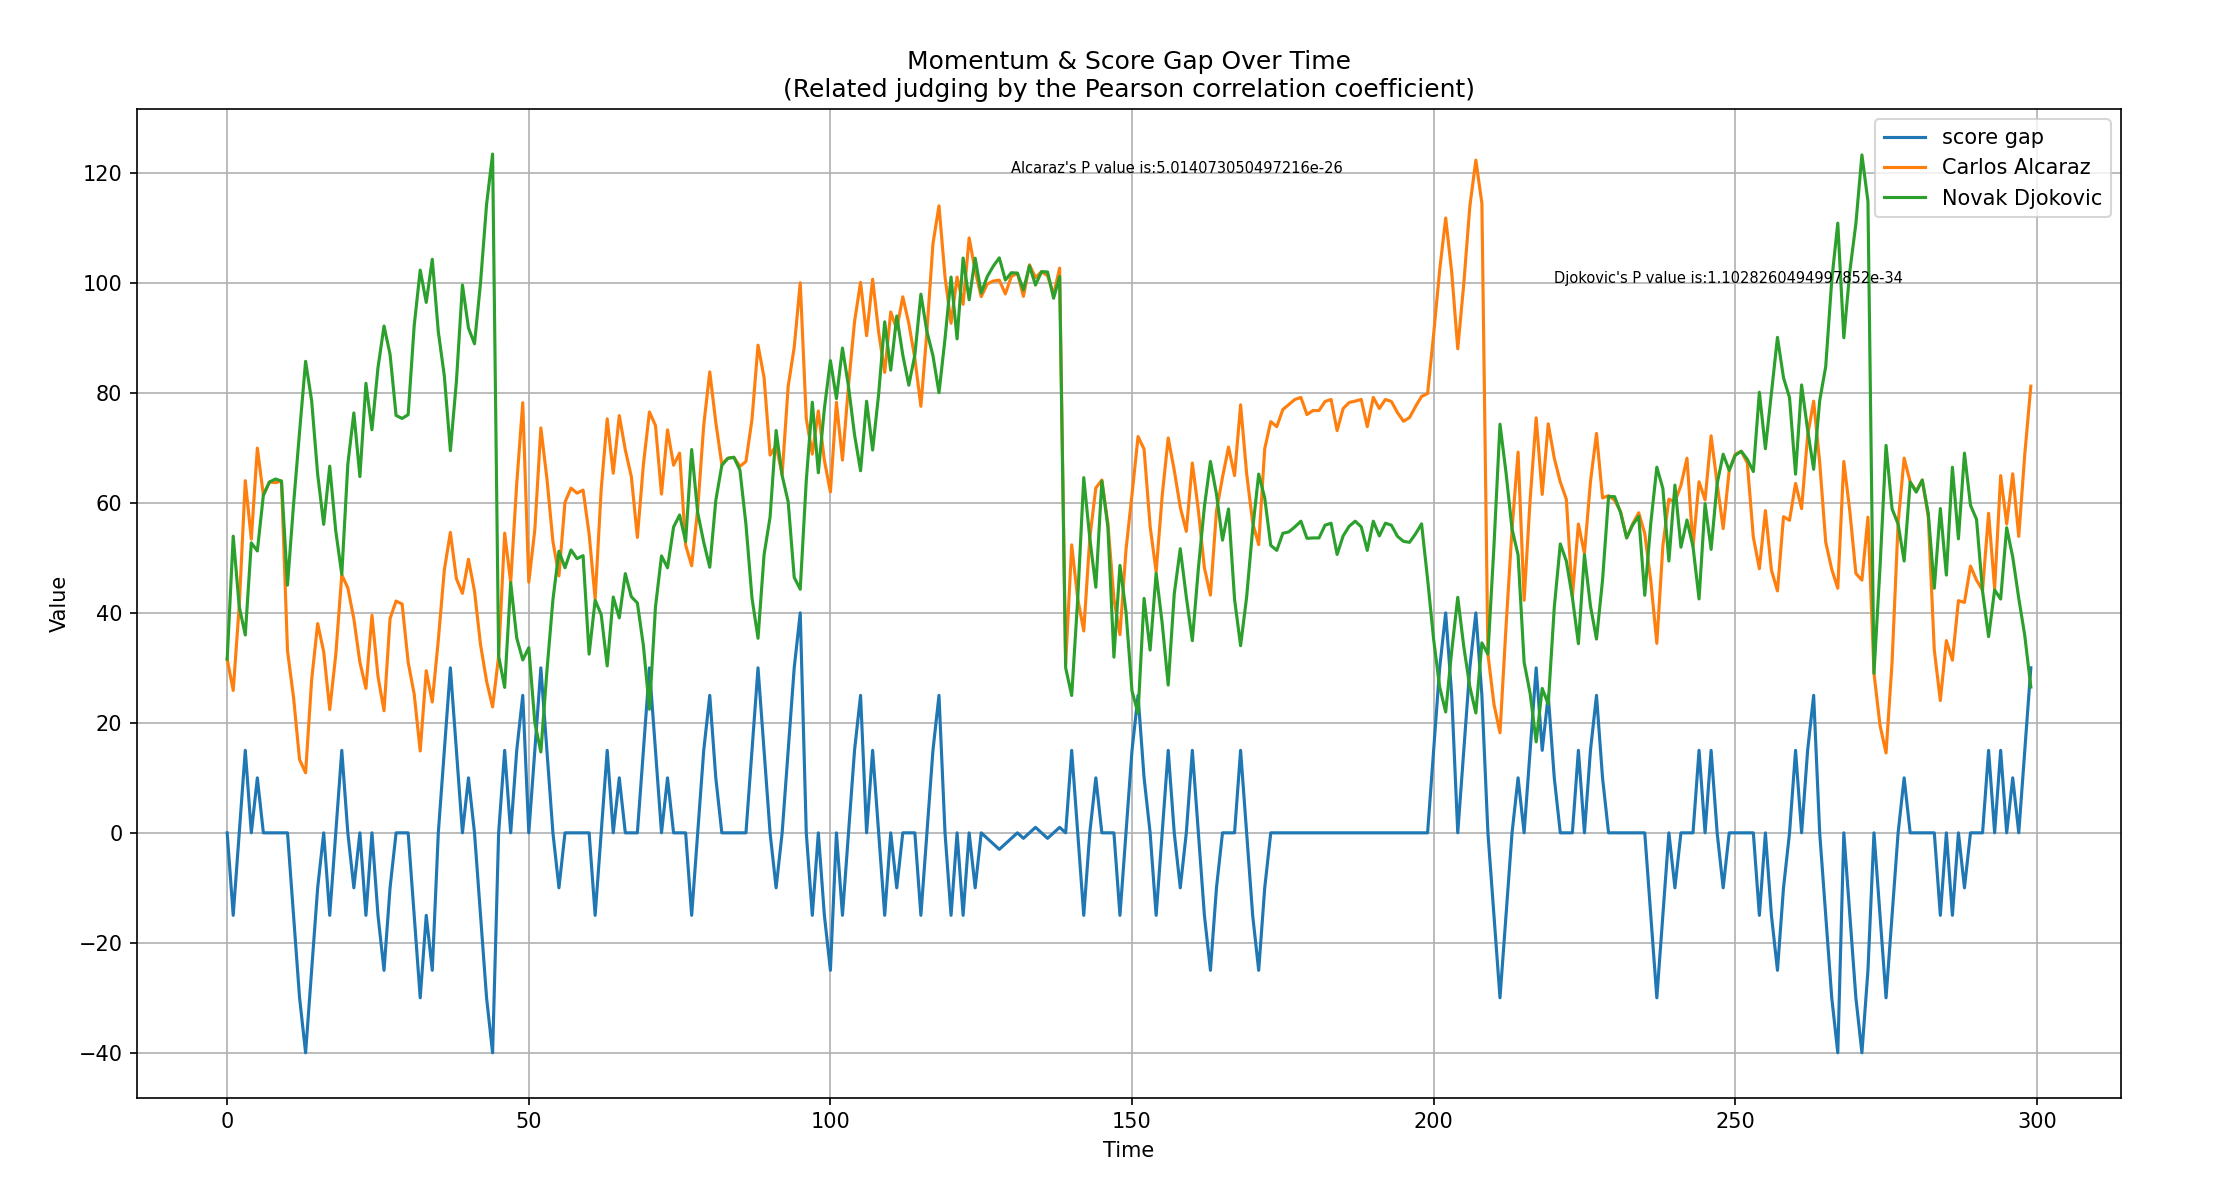
\includegraphics[width=13cm,height=6.5cm]{Further 1.png}
    \caption{Final Momentum Chart} % Title
\end{figure}
\newpage
At the start of the match, Djokovic's momentum was always higher than Alcaraz's, but at times 50 and 100, Alcaraz's momentum began to rise, and Djokovic's momentum underwent a sudden change, and finally Alcaraz's momentum stabilized and surpassed Djokovic's. At the end of the match, even if Djokovic successfully rallied, it was already too late and regrettable. This is why Djokovic lost the match.

Figure 8 is the swing chart of his final with Alcaraz, which can better explain the problem. As can be seen, Alcaraz had a huge momentum boost in the middle of the match, and the red turning point announced the match began to lean towards Alcaraz.
\begin{figure}[h]
	\centering % 居中显示
	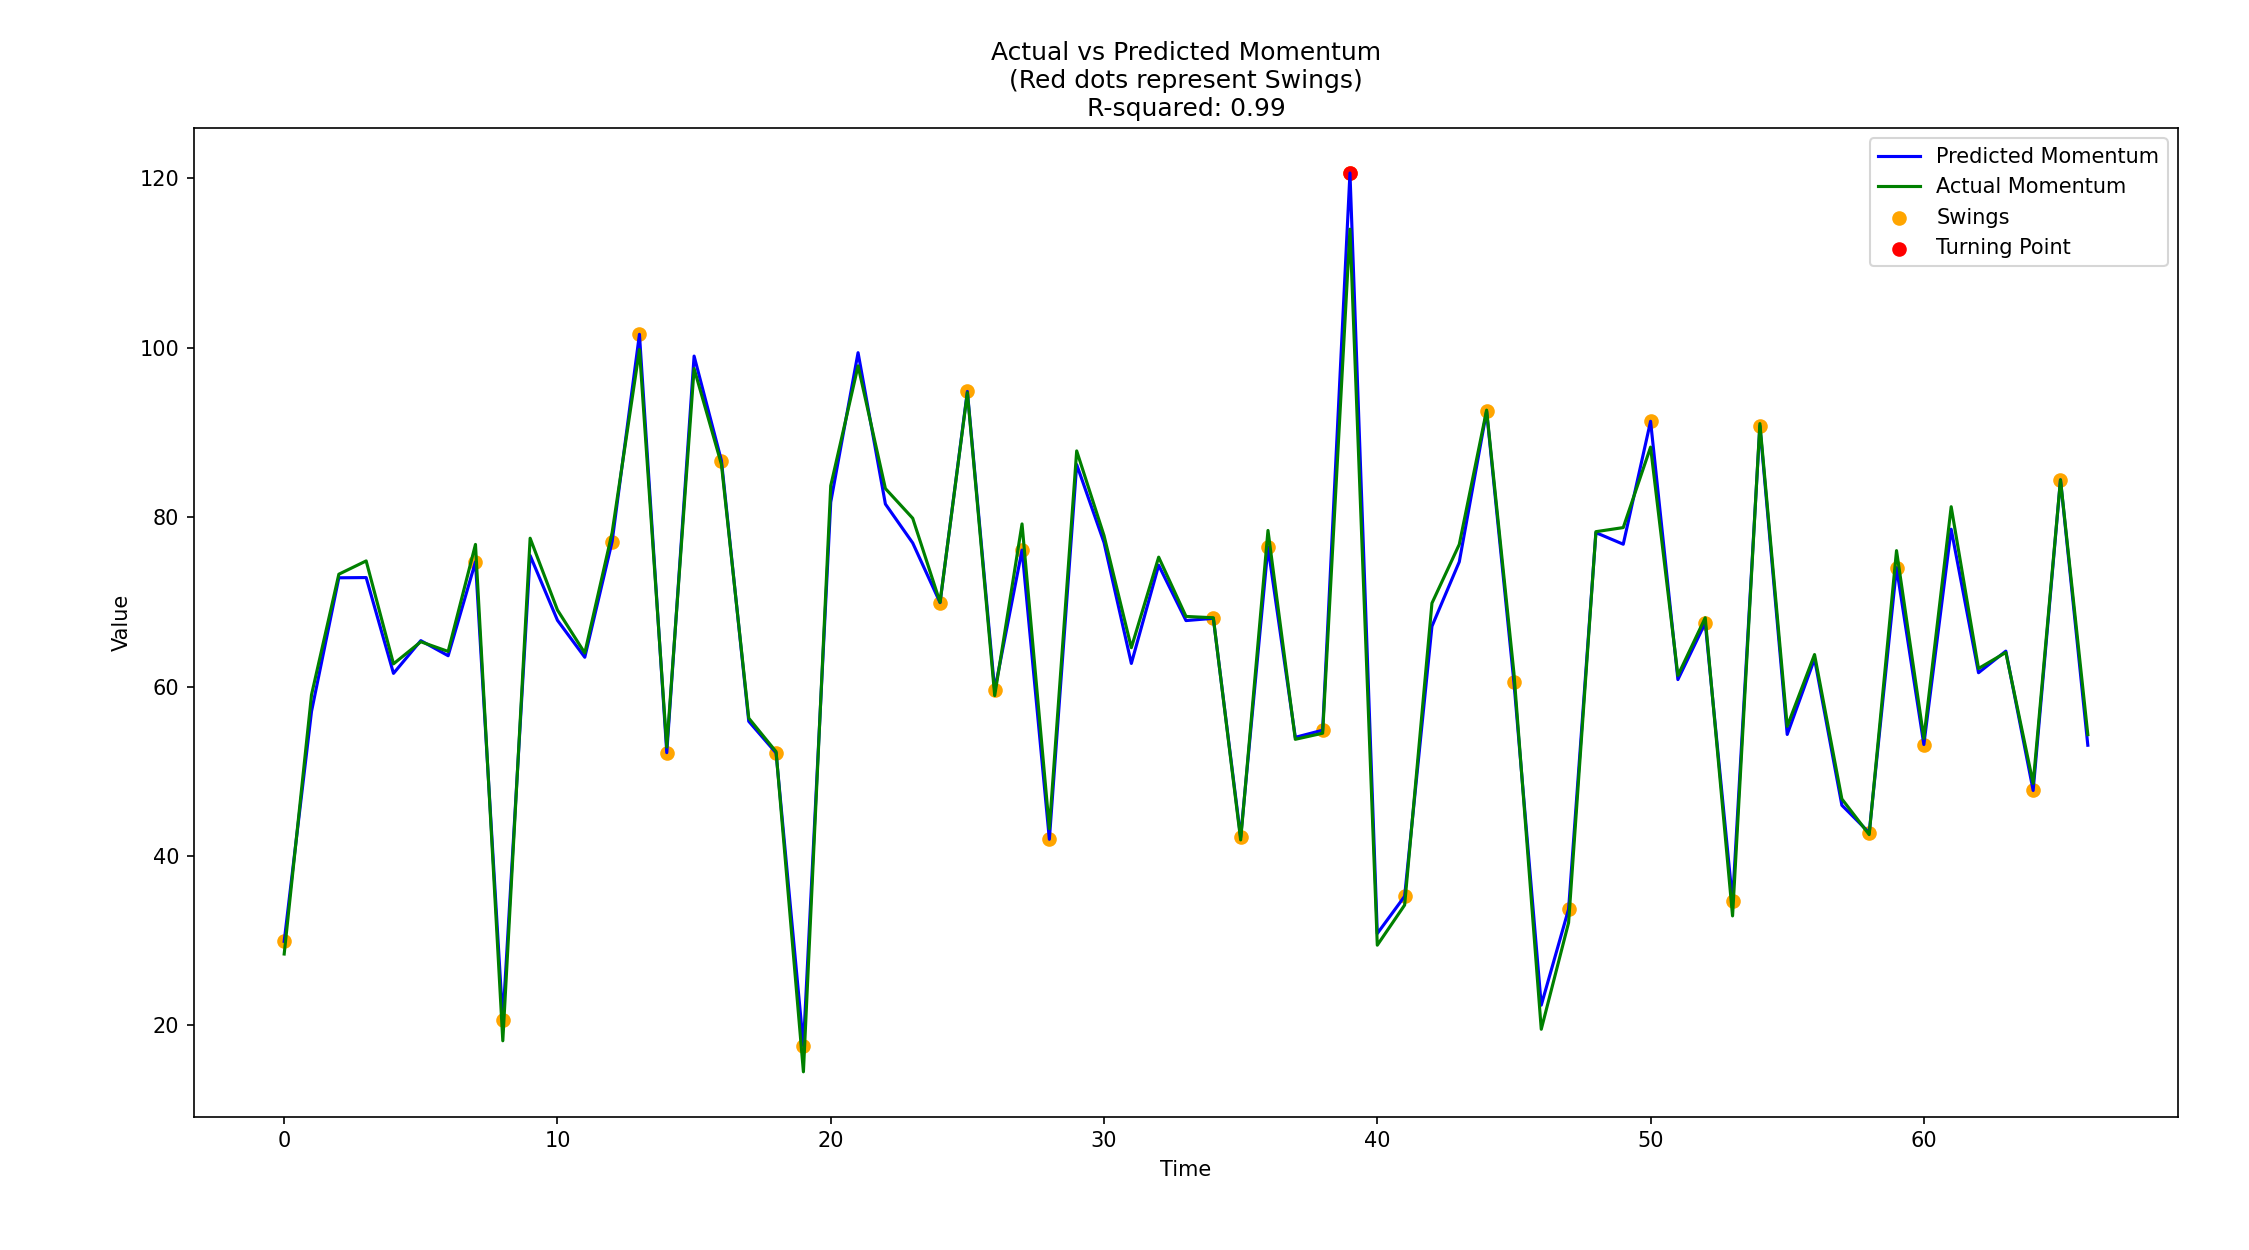
\includegraphics[width=13cm,height=8cm]{Further 2.png}
	\caption{Alcaraz's swings} % 标题
\end{figure}

\begin{wrapfigure}{l}{0.5\textwidth} % "r" for right alignment, "0.5\textwidth" for half of the text width
    \centering
    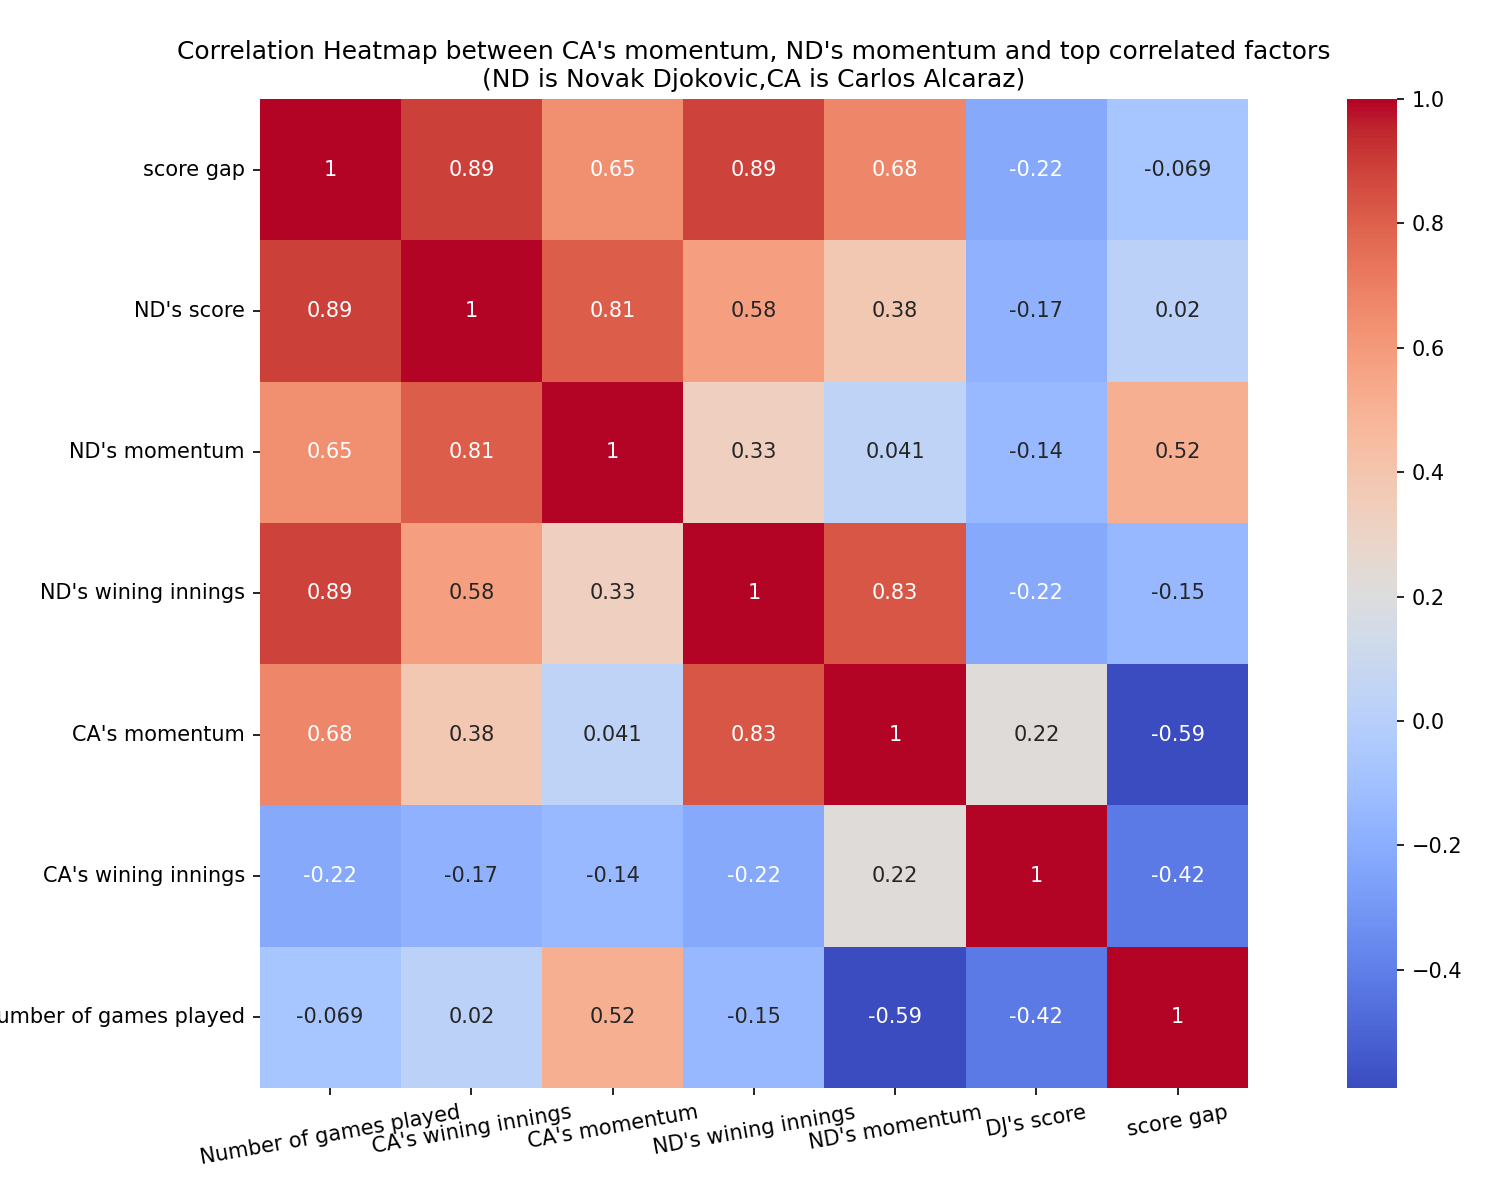
\includegraphics[width=0.38\textwidth]{Further 3.png} % adjust the width as needed
    \caption{Momentum Correlation Heatmap}
\end{wrapfigure}

Finally, let's take a look at the key factors affecting the momentum of the two players.Focus  on the number of games played, and we can see that its correlation with Djokovic's momentum is less than 0, which to some extent, means that Djokovic's momentum has been hit by the number of games played, on the contrary, Alcaraz must have increased. This can also explain Djokovic's failure from one angle.

\textbf{\subsection{Expanding Research}}
Our model's performance in tennis matches has been verified, and the next goal is to extend it to other sports matches, such as table tennis, badminton, and even chess.

In terms of swing prediction, we have adopted sensitivity analysis to enhance the prediction accuracy of the model. In addition, we have also strived to identify a series of auxiliary variables that affect the outcome of the match, including weather conditions, venue quality, and player strength (based on ranking). These factors are incorporated into the prediction model through a weighting method, and then the correlation between each factor and the core prediction factor - "momentum" is evaluated. Furthermore, we have also conducted field visits to sports competition venues, recorded and organized the observations, and formed a detailed dataset. The following are the specific details and analysis results of the collected data.

We utilized available resources to conduct a detailed data analysis of a table tennis match during the winter sports meeting at No.2 High School in Changping District, Beijing, China (player names have been omitted for privacy reasons). The match ultimately ended in a draw. As seen from the momentum chart, the momentum of both players gradually increased as the match progressed, with both hoping to win, resulting in a relatively stable score difference. However, it is difficult to accurately predict the match ending in a draw through the swing chart, which reveals some issues with our model. Regardless, the model can intuitively present the overall performance and swings of the players.

\begin{wrapfigure}{l}{0.5\textwidth} % "r" for right alignment, "0.5\textwidth" for half of the text width
    \centering
    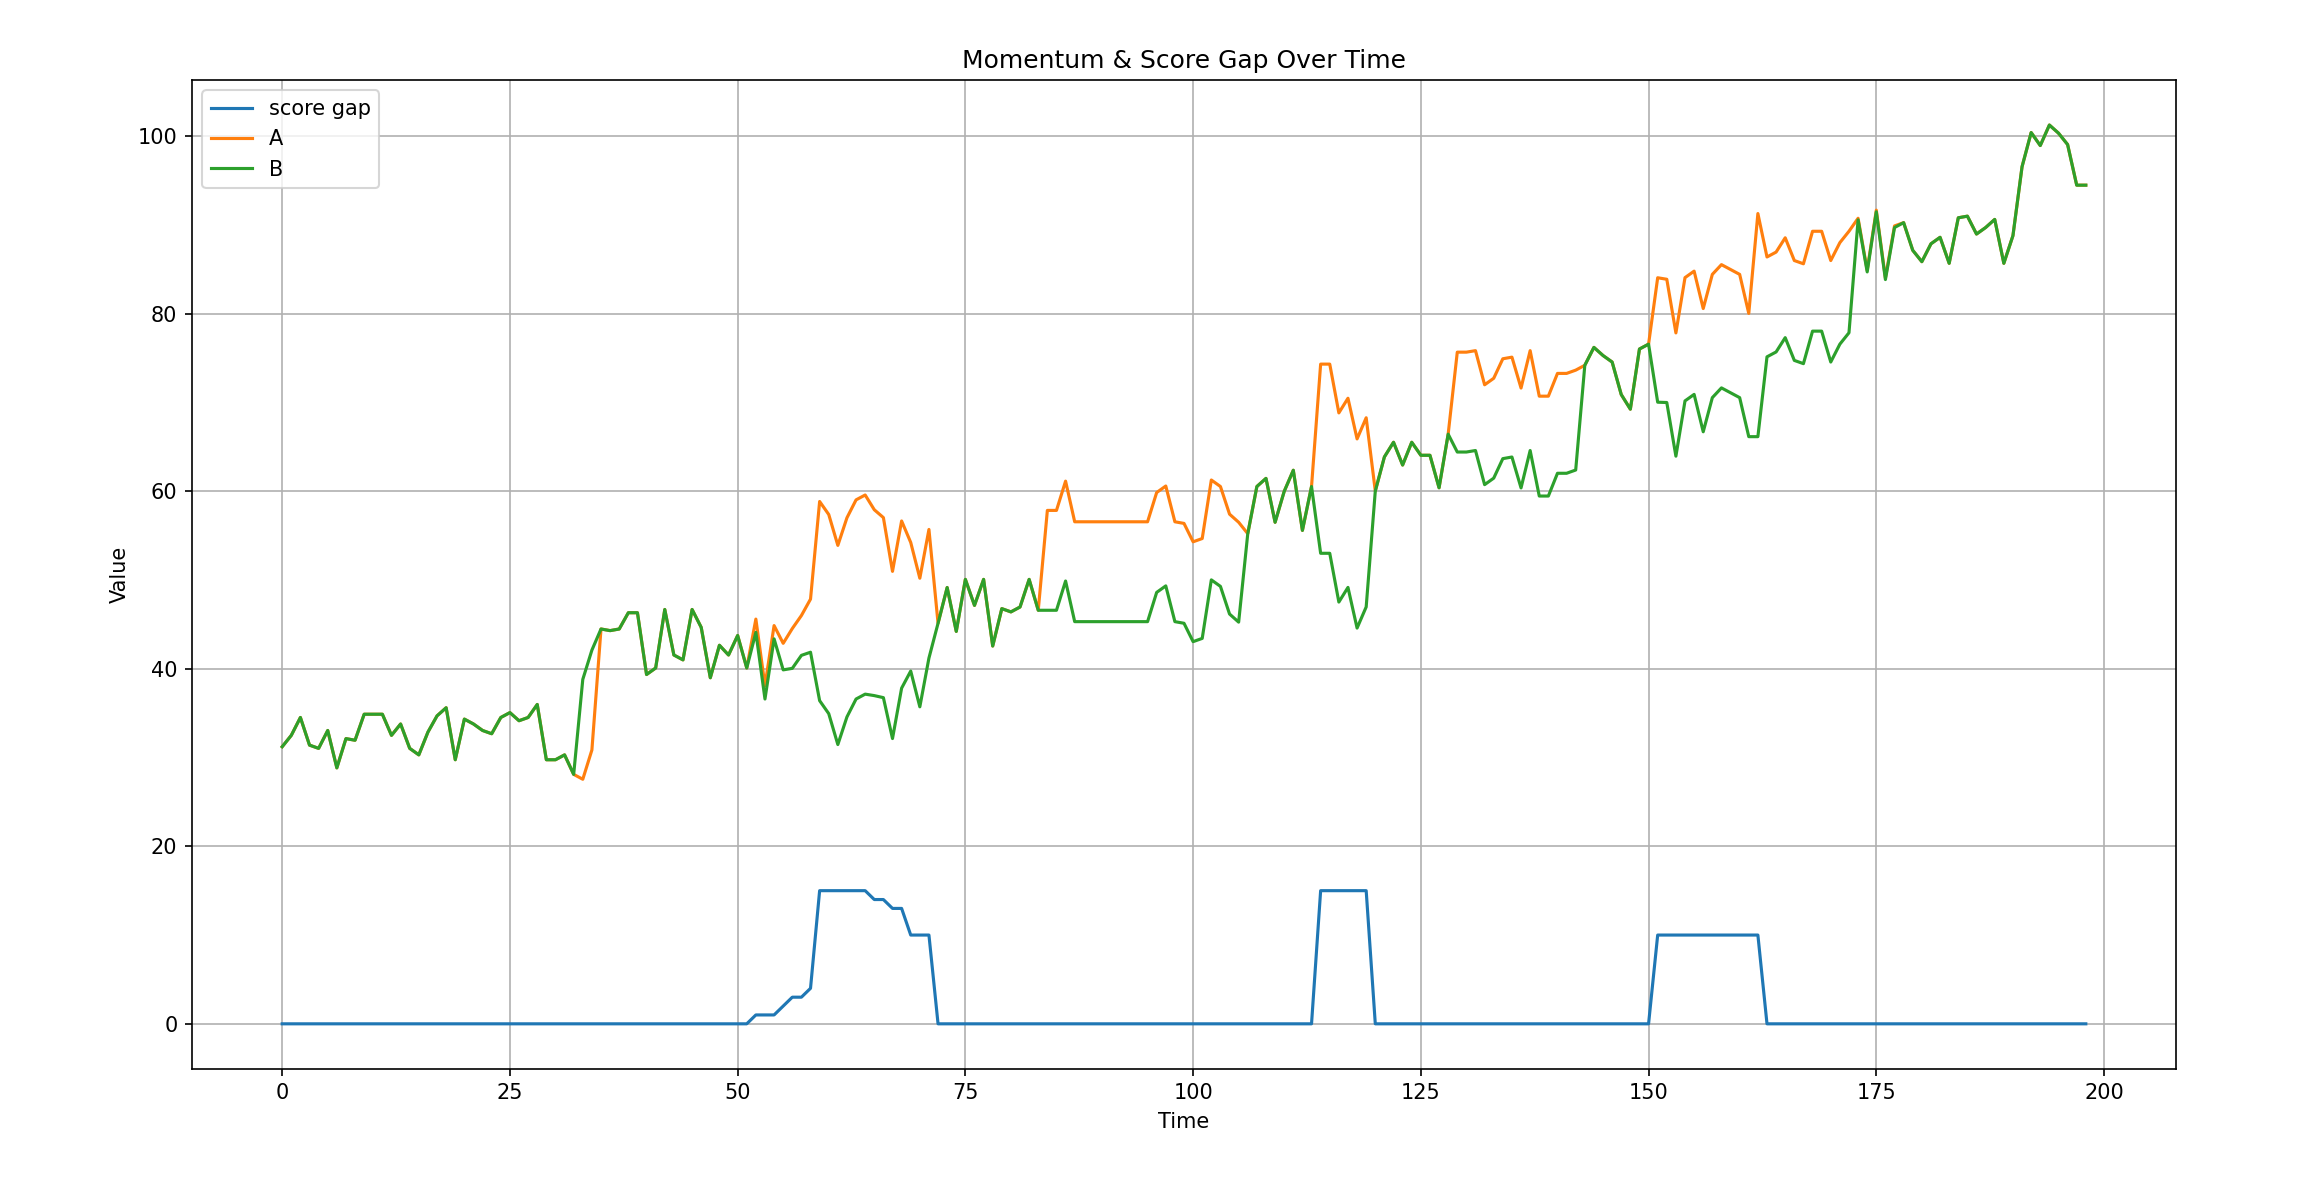
\includegraphics[width=0.33\textwidth]{Expand 1.png} % adjust the width as needed
    \caption{Momentum Chart of Table Tennis Match}
	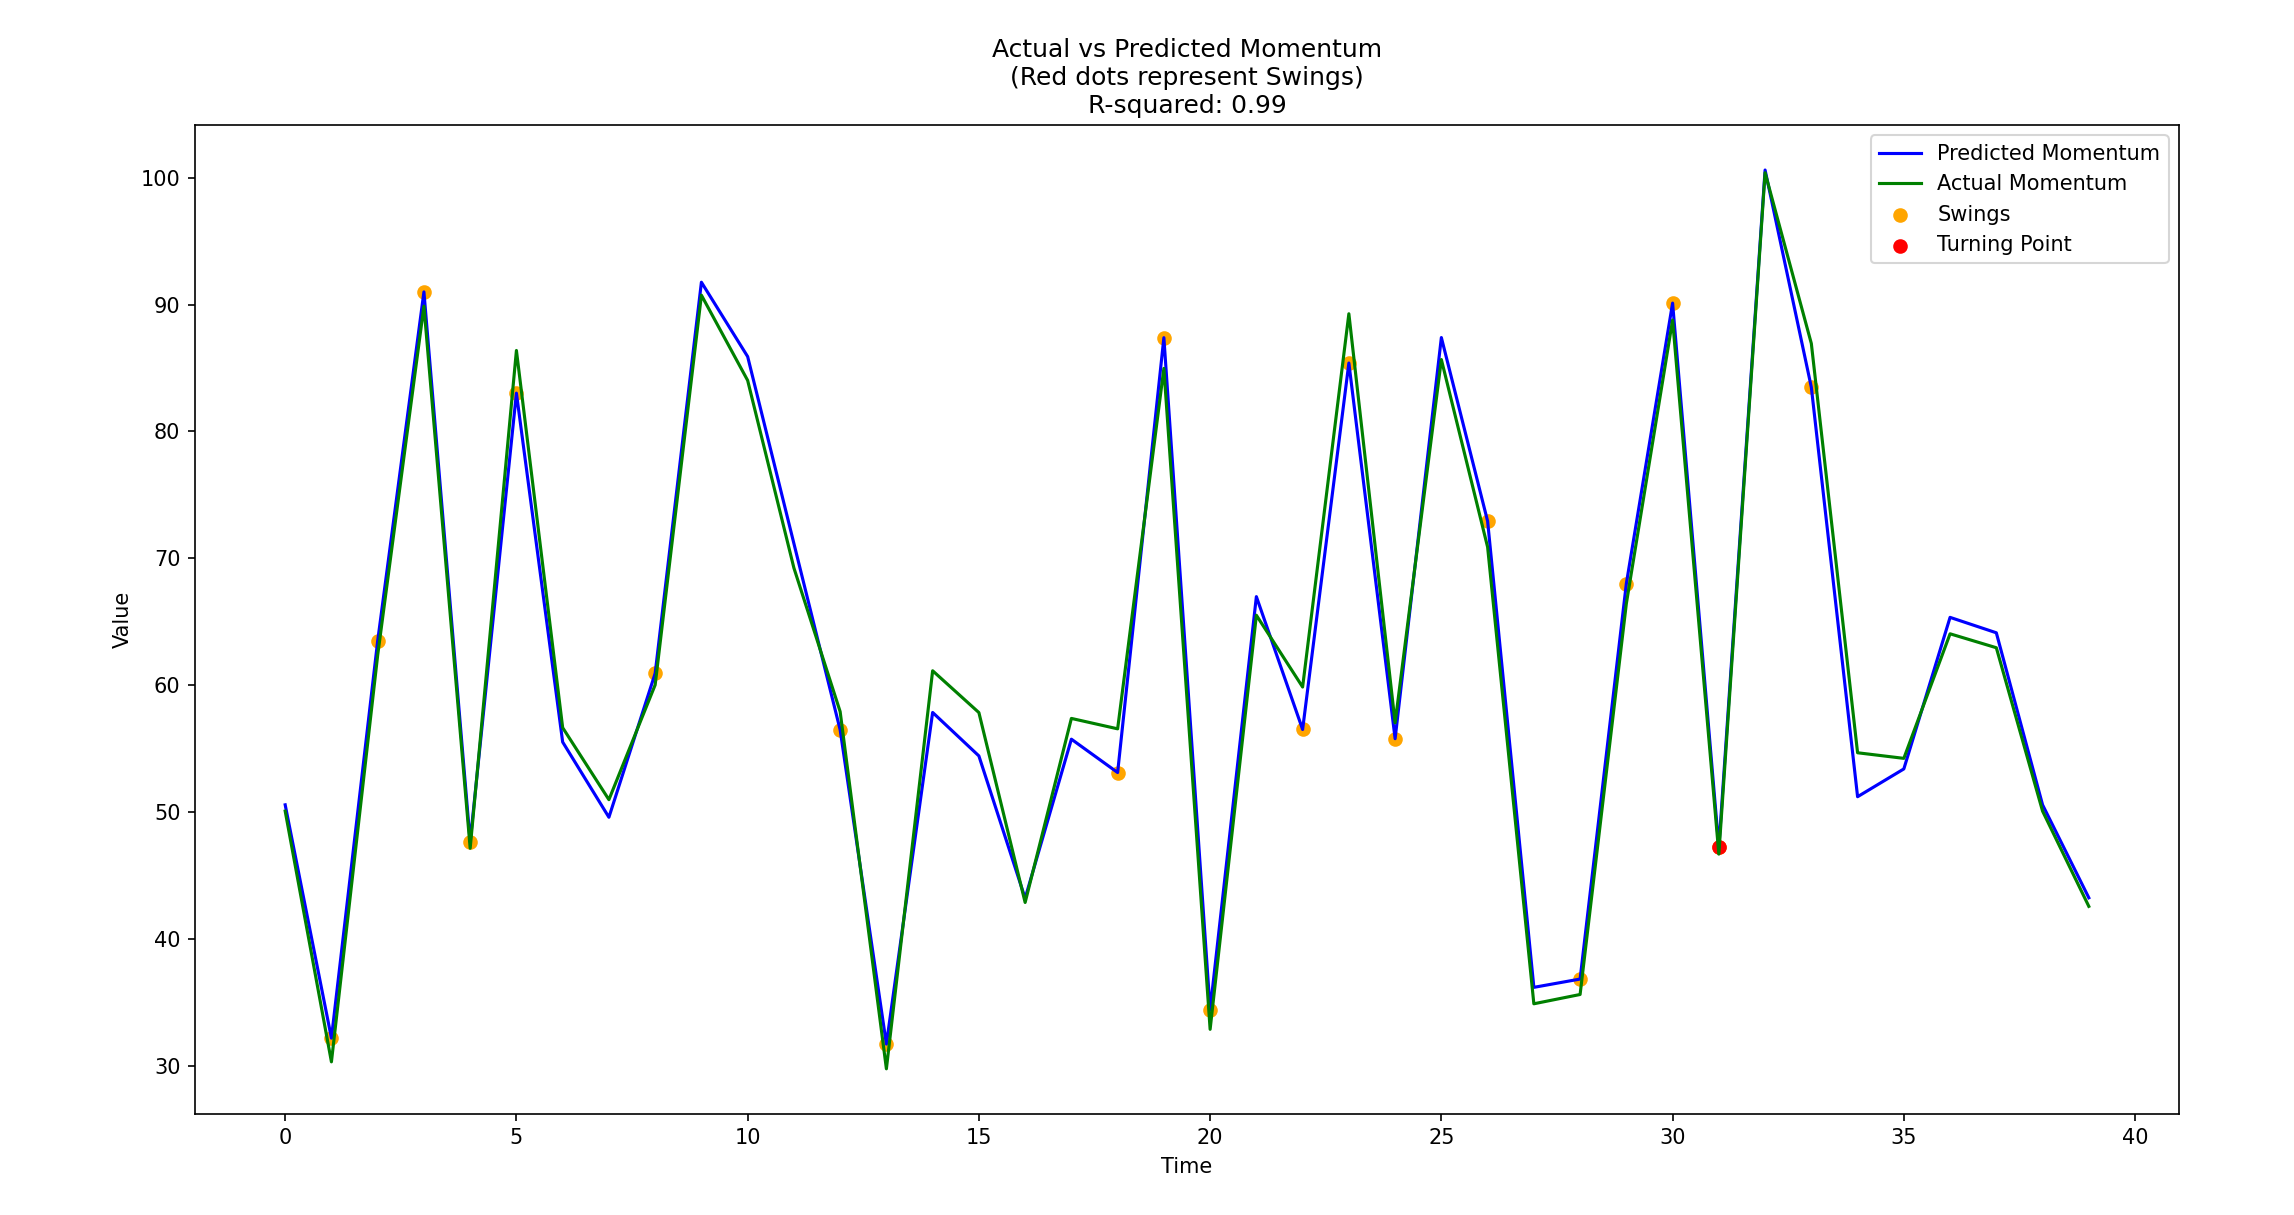
\includegraphics[width=0.33\textwidth]{Expand 2.png}
	\caption{Swing Chart of Table Tennis Match}
\end{wrapfigure}

In addition, through the analysis of the swing chart, we found that the model can still relatively accurately predict momentum changes in more complex environments, and the error is relatively small. This finding confirms the reliability of our model in terms of prediction. In future experiments, we will continue to enhance this advantage.

Through the analysis of this match, we have learned about the strengths and weaknesses of the model, fully demonstrating the model's adaptability to a certain extent in different matches.

\newpage
\textbf{\section{Strengths and Weaknesses}}
\textbf{\subsection{Strengths}}
\begin{itemize}
	\item In our model, we utilize various visualizations, including scatter plots, line charts, and heat maps, to analyze the impact of momentum on the performance of players. These visuals provide intuitive results for further analysis, contributing to a concise, easy-to-understand yet powerful model structure. Our model can also be applied to other competitions, such as table tennis matches, demonstrating strong generalizability.
	\item By using the Momentum-Swings Prediction Model, our model simulates momentum changes, predicts swings, and effectively forecasts turning points in the competition.
	\item Our model boasts an impressive training speed, not only excelling in data learning but also providing users with a more efficient user experience, saving a significant amount of time.
\end{itemize}

\textbf{\subsection{Weaknesses}}
\begin{itemize}
	\item For the sake of enhanced comprehensibility and computational simplicity, we make the assumption that the data follows a linear pattern. In reality, due to various influencing factors, the actual scenario might exhibit non-linear characteristics, posing the potential risk of inaccuracies in the model.
	\item Our model exhibits a heightened sensitivity to outliers, and instances where there are significantly deviant anomalies may potentially result in the instability of the model.
\end{itemize}

\newpage
\textbf{\section{Stability Analysis}}
We used the LSTM (Long Short-Term Memory) [3] test to quantify the stability of the model. LSTM is a type of long short-term memory network, which is a special type of RNN (Recurrent Neural Network). Compared with traditional RNNs, LSTM is more suitable for processing and predicting important events with long intervals in time series. The standard LSTM structure includes four parts: memory cell, input gate, output gate, and forget gate.
\begin{itemize}
    \item Memory cell: Responsible for storing information.
    \item Input gate: Responsible for deciding which information can pass and which cannot.
    \item Output gate: Responsible for deciding which information can be output.
    \item Forget gate: Responsible for deciding which information needs to be forgotten.
\end{itemize}
We used the simplified GRU algorithm, which removed the input gate and combined the operations of the input gate and forget gate in the reset gate.

The test included 100 sets of data, and the results are shown in Figure 12.

\begin{figure}[h]
    \centering % Centered display
    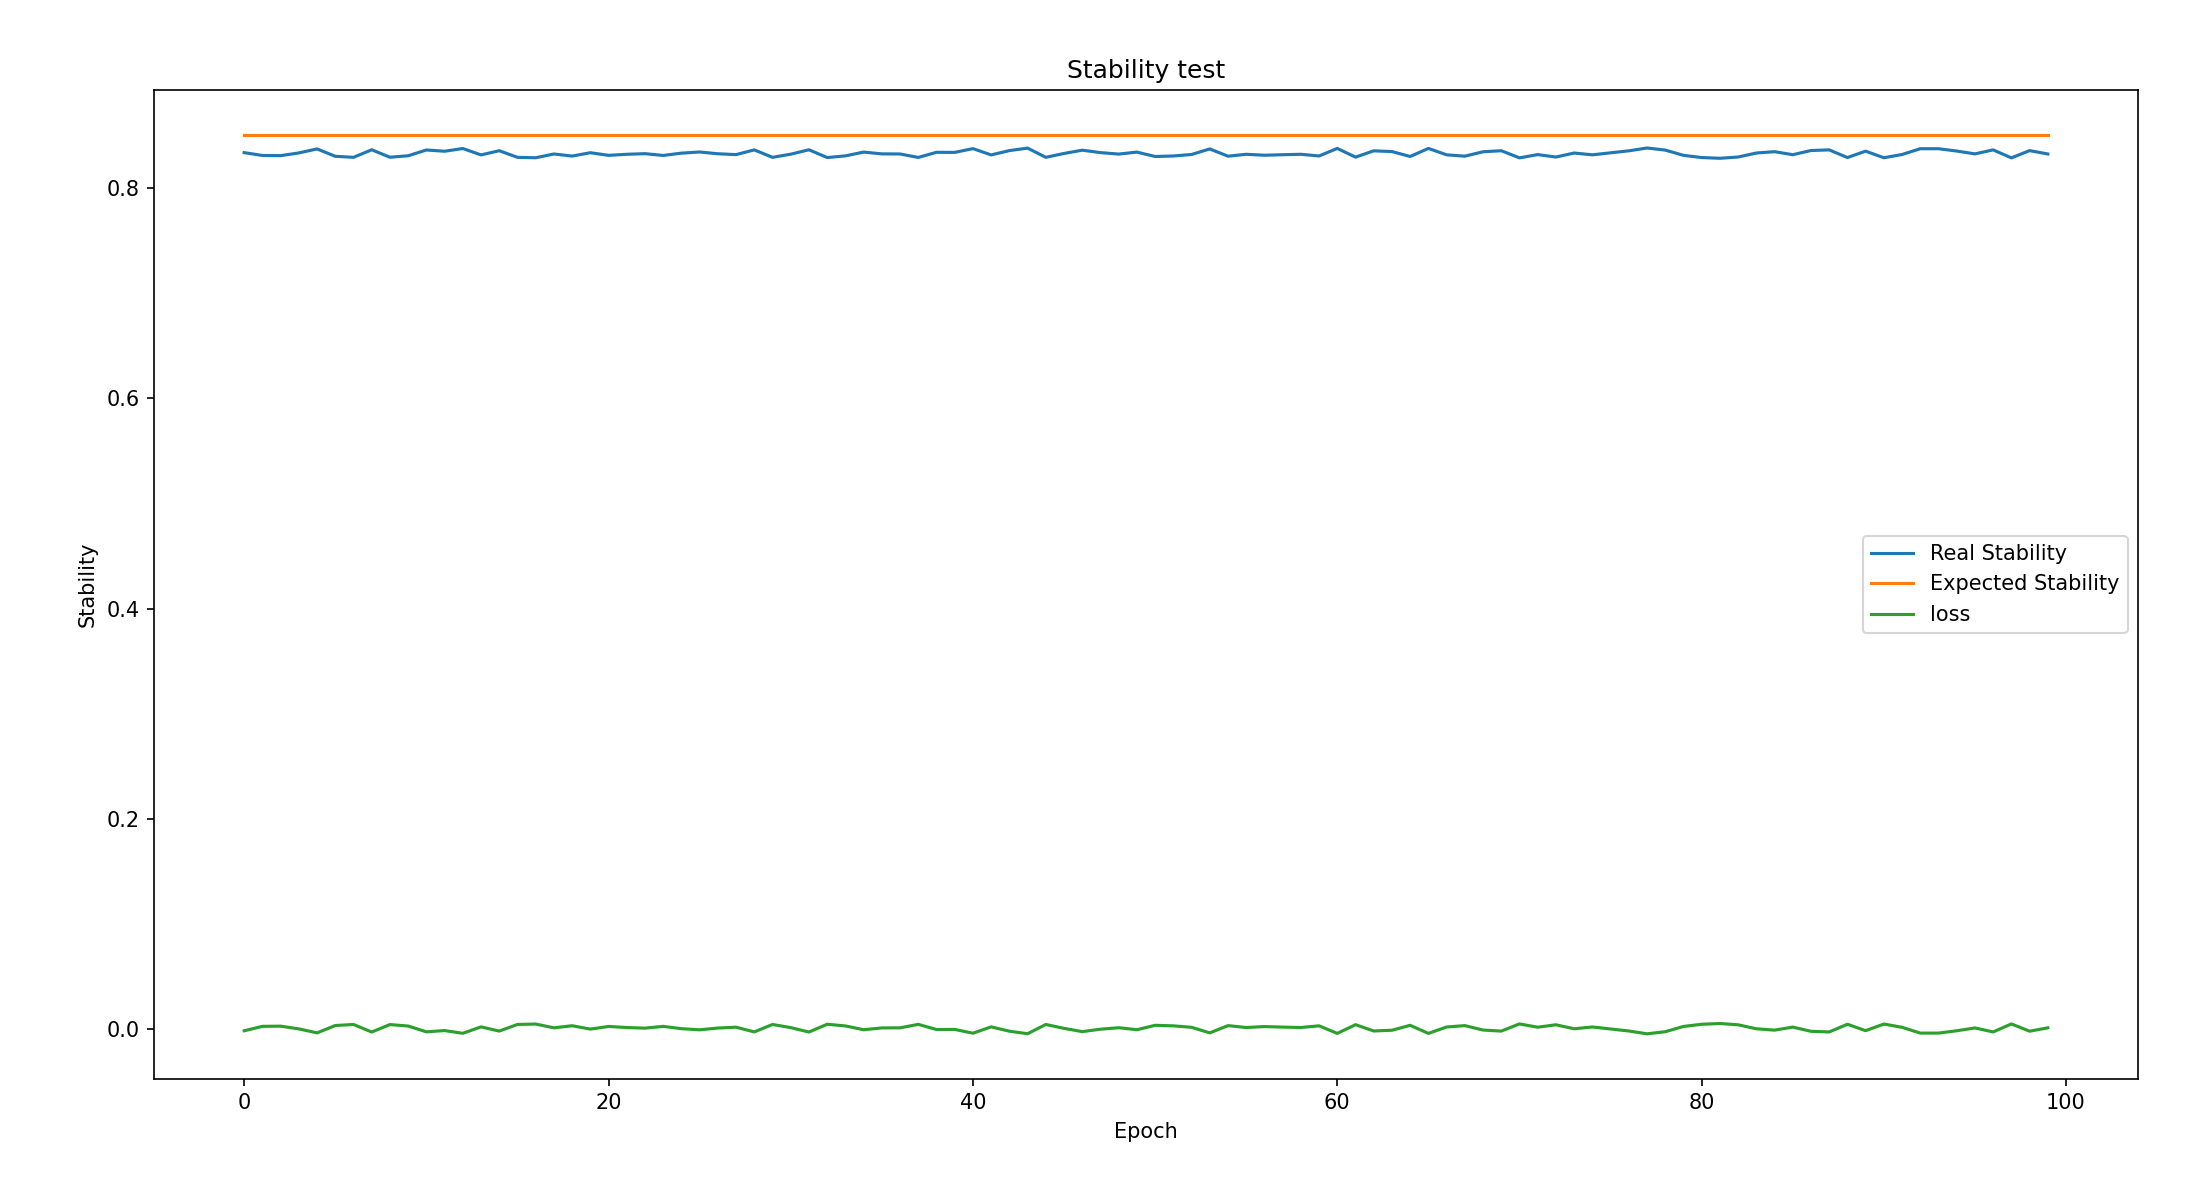
\includegraphics[width=12cm,height=6cm]{Stability test.png}
    \caption{Stability test} % Title
\end{figure}

We found that the actual accuracy value is close to the predicted accuracy value, and the loss is kept at a low level, indicating that the model has successfully passed the stability test.

\textbf{\section{Conclusion}}
We have established a model to analyze the data of the entire match and determine the levels of the players involved. We have quantified the concept of "momentum" to gauge potential swings during the match, conducting a comprehensive analysis of its correlation with player performance. Utilizing the data, we predict the timing of the match's momentum shifts and further test the stability of the model with a broader range of matches. Here are some of our intriguing findings:
\begin{itemize}
	\item The player's skill and mentality should both be considered as part of the momentum. Momentum is not constant; it undergoes various changes, such as when a player scores a winning point or makes a significant mistake. This not only affects the player's psychology but may also have certain implications for their skill.
	\item Swings are strongly correlated with the success of players, and the changes in momentum are also one of the necessary conditions for generating swings.
	\item Due to the varying strengths and psychological factors of players, each game will have unpredictable and random situations. Therefore, changes in momentum are to some extent normal, but significant shifts in momentum often accompany reversals in the course of the game.
\end{itemize}

% 因为不输出此部分到目录 \addcontentsline{}{}{}是添加此标题到目录 
\newpage
\textbf{\section*{References}\addcontentsline{toc}{section}{References}}
\begin{enumerate}[label={【\arabic*】}]
	\item  Merriam-Webster Dictionary: Momentum,\\\url{https://www.merriam-webster.com/dictionary/momentum}
	\item  Wikipedia: Pearson correlation test,\\\url{https://en.wikipedia.org/wiki/Pearson_correlation_coefficient}
	\item  Amazing Adoo, Basic Knowledge of LSTM,\\\url{https://zhuanlan.zhihu.com/p/598124702}
\end{enumerate}

\newpage
\textbf{\section*{Appendice}\addcontentsline{toc}{section}{Appendice}} 
\fontsize{13pt}{12.5pt}\selectfont
Here is a picture describing LSTM/GRU and some of codes we used in our model, which python is the main development language.
\vspace{7pt}
\textbf{\subsection*{Appendice A: What is LSTM/GRU?}}
\begin{figure}[h]
	\centering % Centered display
	
\includegraphics[width=8cm,height=10cm]{LSTM.png}
	\caption{LSTM/GRU} % Title
\end{figure}

\textbf{\subsection*{Appendice B: Momentum Changes and Swings Prediction}}
\noindent{\rule{\textwidth}{0.2mm}}
\vspace{-18pt} 
\fontsize{8pt}{7.5pt}\selectfont
{
	\lstinputlisting[language=python]{Appendix.py}
}
\vspace{-12pt}
\noindent{\rule{\textwidth}{0.3mm}}


\noindent{\rule{\textwidth}{0.3mm}}
\end{document}